%   \label{sec:signalIndependentLimits}% uncomment if label used. 
%\subsubsection{Untagged Resonances: Model-independent Gaussian Limits}
%       \label{subsec:UntaggedResonancesGaussianLimits} % uncomment if label used. 


Given that no significant deviation from the expected background is observed, the limits derived on several signal models that could cause a resonance in the dijet invariant mass distribution through a frequentist approach. For the 1-$g$ tagged and 2-$g$ tagged categories, the upper limits are set on the signal cross-section times acceptance times gluon-tagging selection efficiency times branching ratio.  The anticipated limits are determined using the asymptotic approximation of the test statistic's distribution, complemented by pseudo-experiments shaped by the background uncertainty values from the maximum-likelihood fit. For signal interpretations in the high-mass regions where the relative discrepancy from the asymptotic approximation exceeds 1\%, pseudo-experiments are utilized. The derived limits undergo logarithmic interpolation. No variations are made to the theoretical cross-sections of the signal. Both background and signal sample systematic uncertainties are factored into the limits by adjusting all sources of uncertainty based on Gaussian probability distributions. In the context of the signal models assessed, the couplings of the new physics resonance are notably strong relative to the perturbative QCD scale at the given signal mass, rendering interference with QCD components negligible.


The upper limits obtained from all categories are shown in Figures~\ref{fig:SignalIndependentGaussianLimits_UntaggedYStar0p8}, and on QBH models are given in Figures~\ref{fig:SignalIndependentGaussianLimits_UntaggedYStar0p81}. The observed limit in 2-$g$ tagged region gives higher \mjj\ than that in 1-$g$ tagged and untagged regions. Table~\ref{tab:0g} provides a summary of the signal masses corresponding to the lower limits for each benchmark model under consideration in untagged region, whereas Table~\ref{tab:1g} for 1-$g$ tagged and Table~\ref{tab:2g} for  2-$g$ tagged region. The analysis incorporating gluon-tagging gains significantly from enhancements in the high transverse momentum q/g-jet classification algorithm. This leads to a boost in sensitivity that surpasses what would be anticipated solely from the increase in integrated luminosity.



        \begin{figure}[!htb]
	            \subfloat[]{ 
		%             label{fig:SignalIndependentGaussianLimits_SubWidth0} % uncomment if label used. 
		                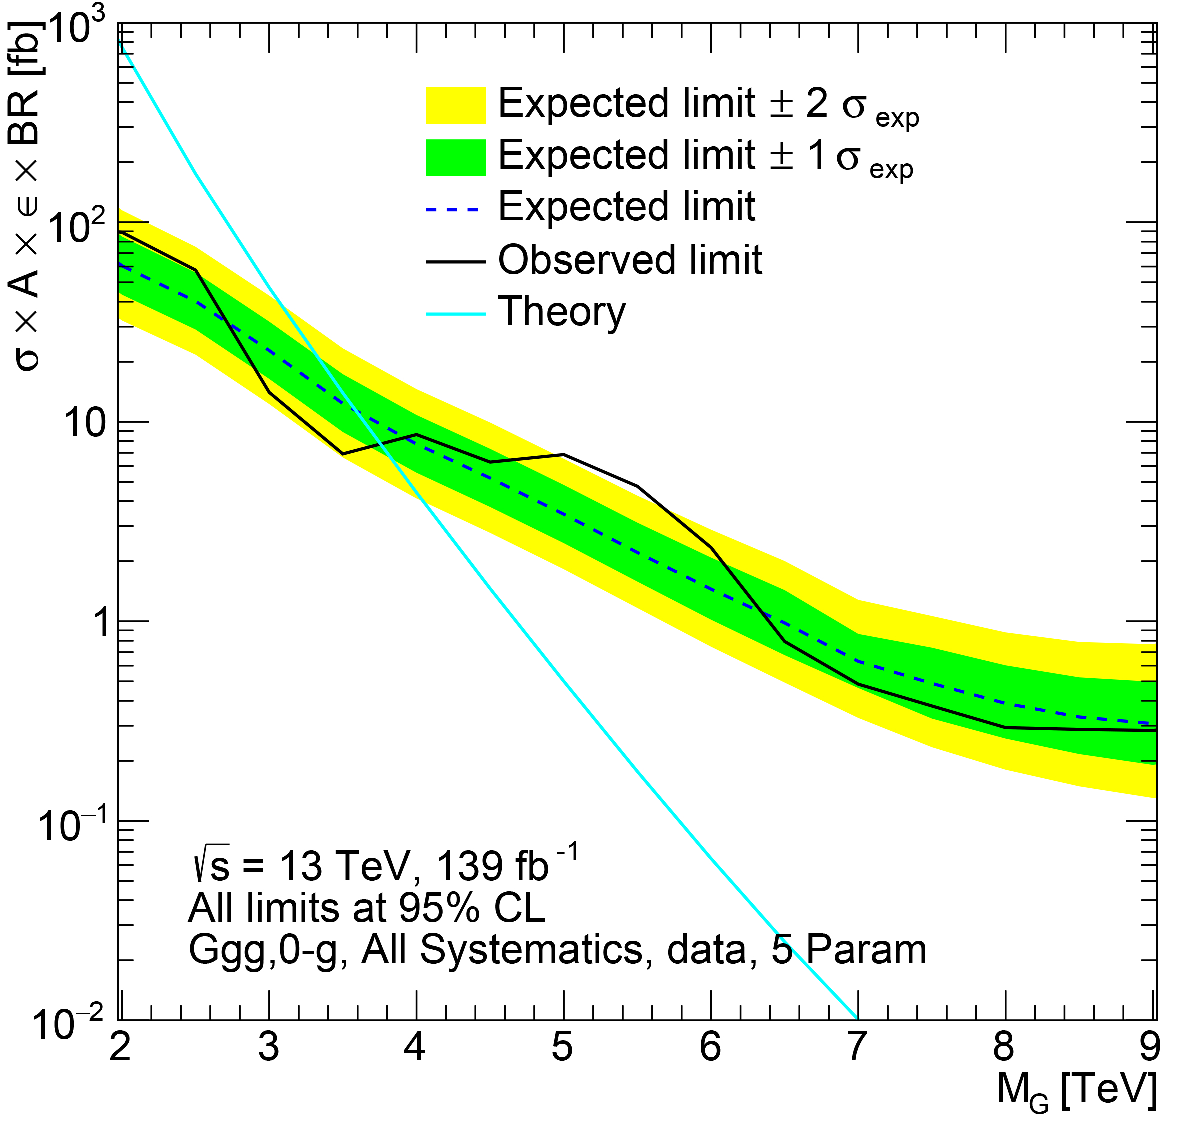
\includegraphics[width=0.45\textwidth]{fig/new_Limit/Ggg_Tag0_yStar0p8_data1_Set1_Param5_LumiSyst0p0083_JESJERtrue_sigma.pdf}
		            }
	            \subfloat[]{ 
		%                \label{fig:SignalIndependentGaussianLimits_SubWidth3} % uncomment if label used. 
		                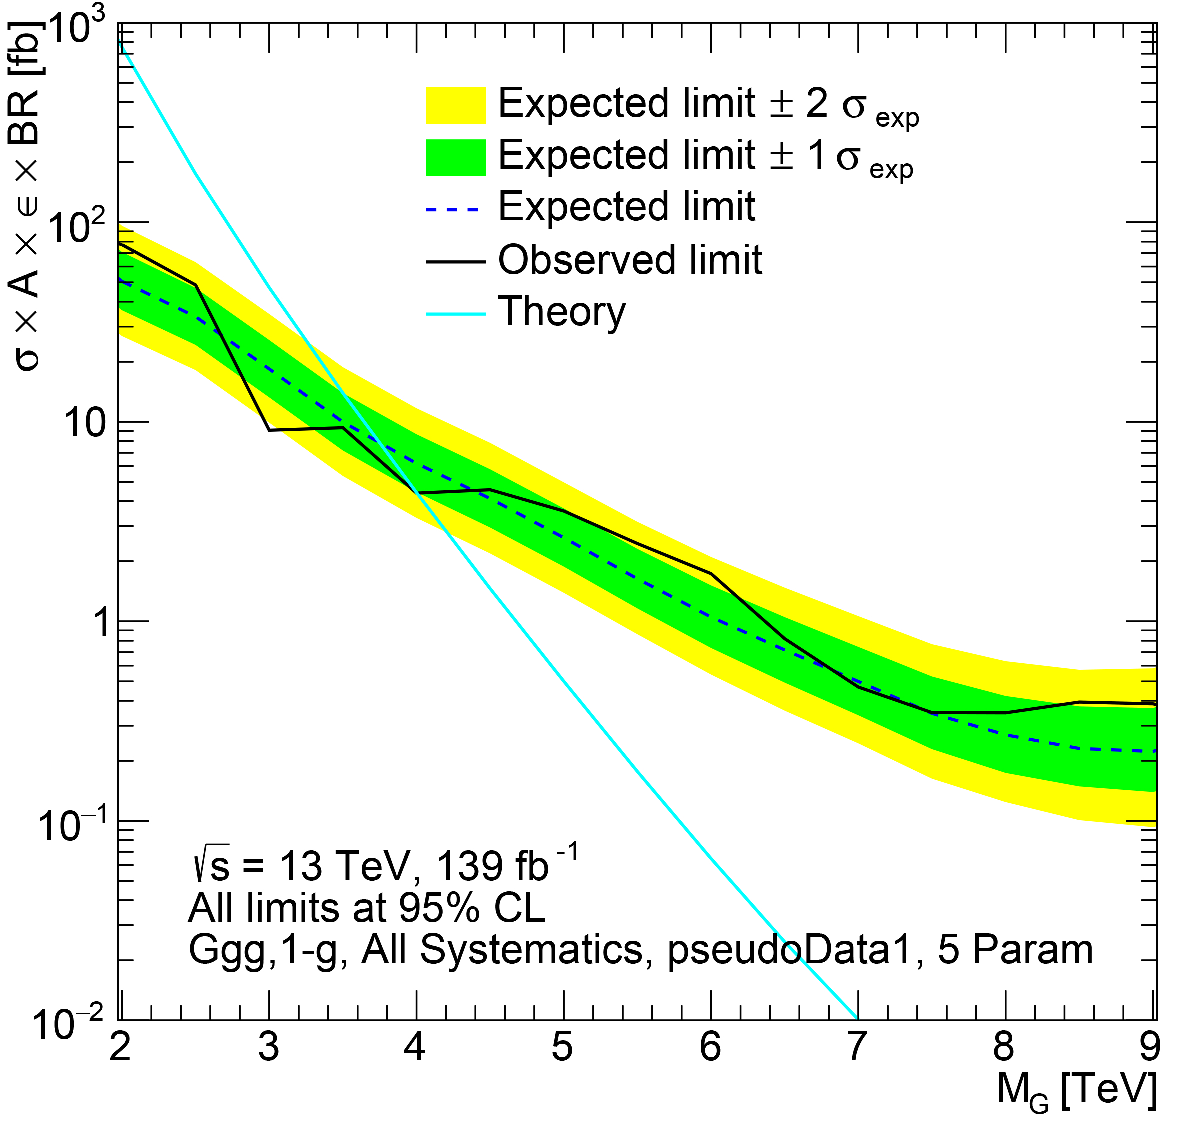
\includegraphics[width=0.45\textwidth]{fig/new_Limit/Ggg_Tag1_yStar0p8_data0_Set1_Param5_LumiSyst0p0083_JESJERtrue_sigma.pdf}
		            }\\
	            \subfloat[]{ 
		%                \label{fig:SignalIndependentGaussianLimits_SubWidth5} % uncomment if label used. 
		                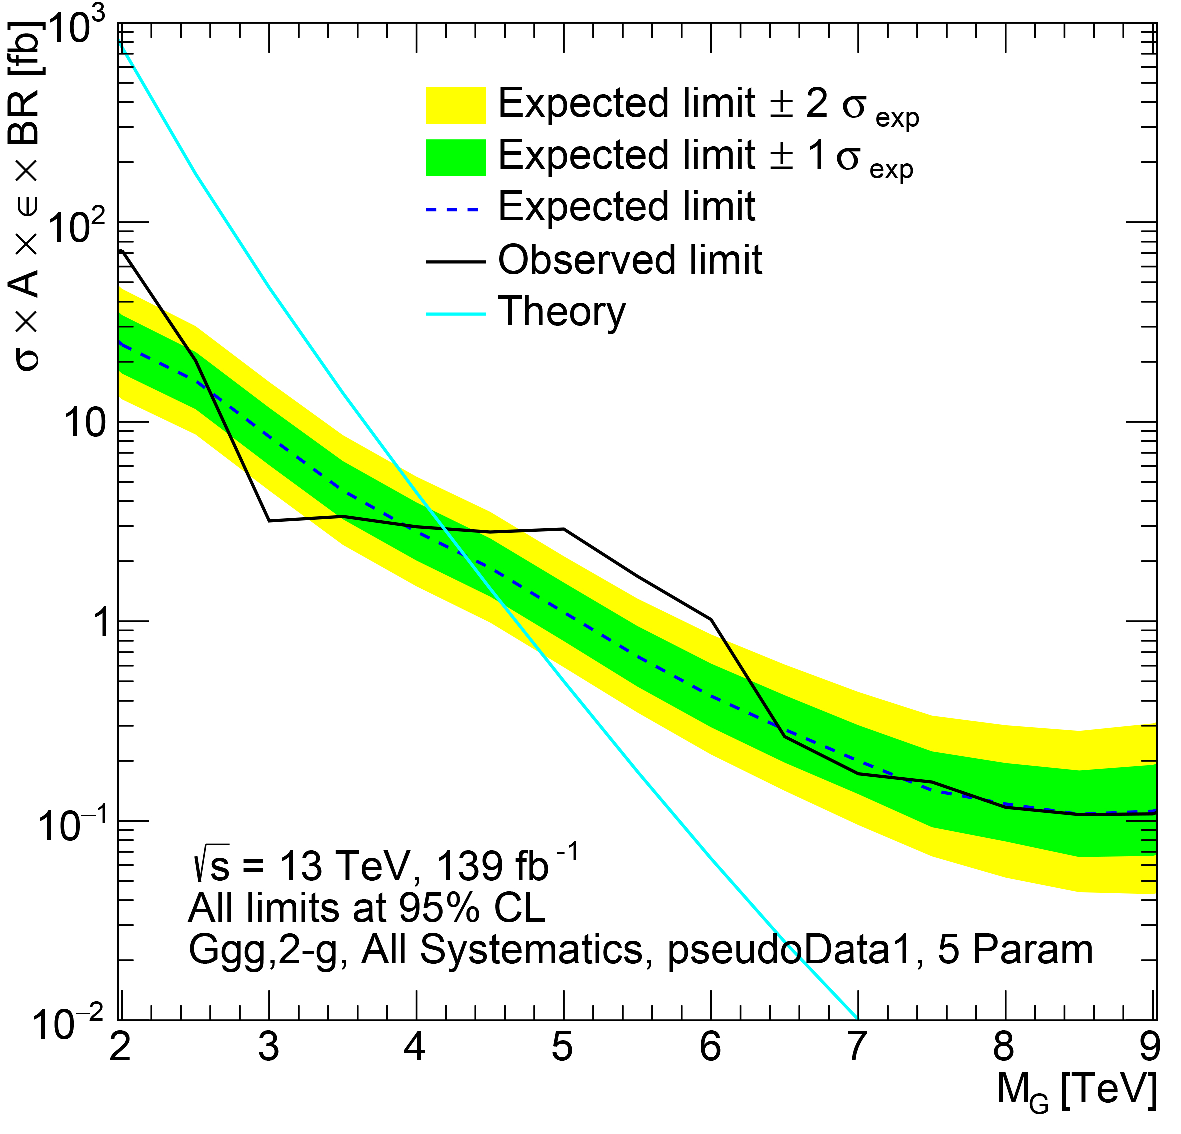
\includegraphics[width=0.45\textwidth]{fig/new_Limit/Ggg_Tag2_yStar0p8_data0_Set1_Param5_LumiSyst0p0083_JESJERtrue_sigma.pdf}
		            }
	            \caption{Upper limits set in the untagged (a),  1-$g$ tagged (b) and 2-$g$ (c) tagged Signal Region using Graviton model with systematics included using the full 139 fb$^{-1}$ Run-2 dataset.}
	            \label{fig:SignalIndependentGaussianLimits_UntaggedYStar0p8}
	  \end{figure}
          \begin{figure}[!htb]
  	\subfloat[]{ 
  		%             label{fig:SignalIndependentGaussianLimits_SubWidth0} % uncomment if label used. 
  		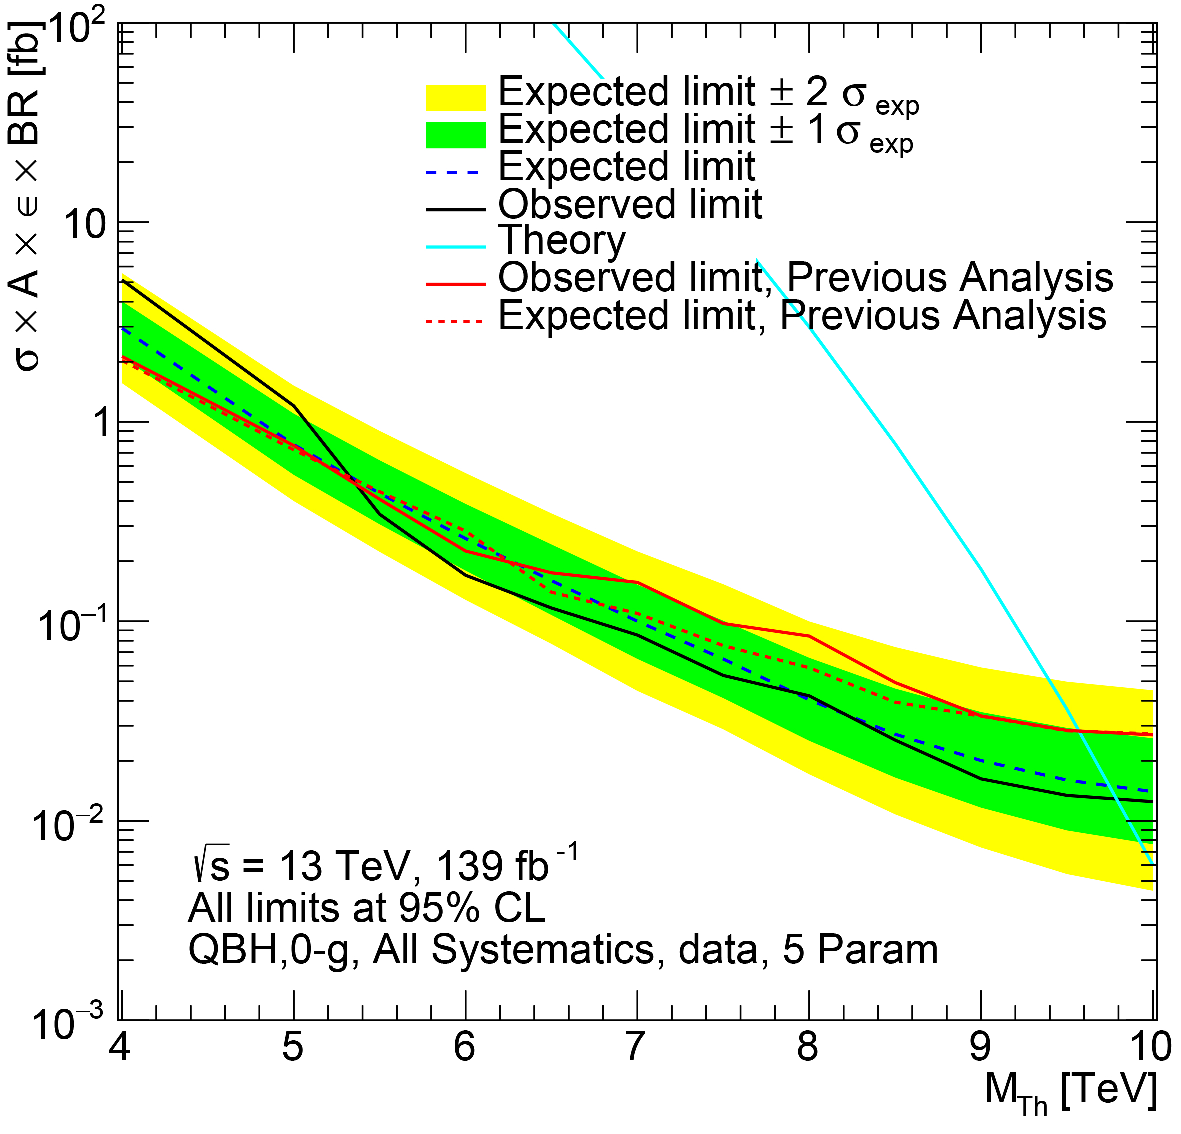
\includegraphics[width=0.45\textwidth]{fig/new_Limit/QBH_Tag0_yStar0p8_data1_Set1_Param5_LumiSyst0p0083_JESJERtrue_sigma.pdf}
  	}
  	\subfloat[]{ 
  		%                \label{fig:SignalIndependentGaussianLimits_SubWidth3} % uncomment if label used. 
  		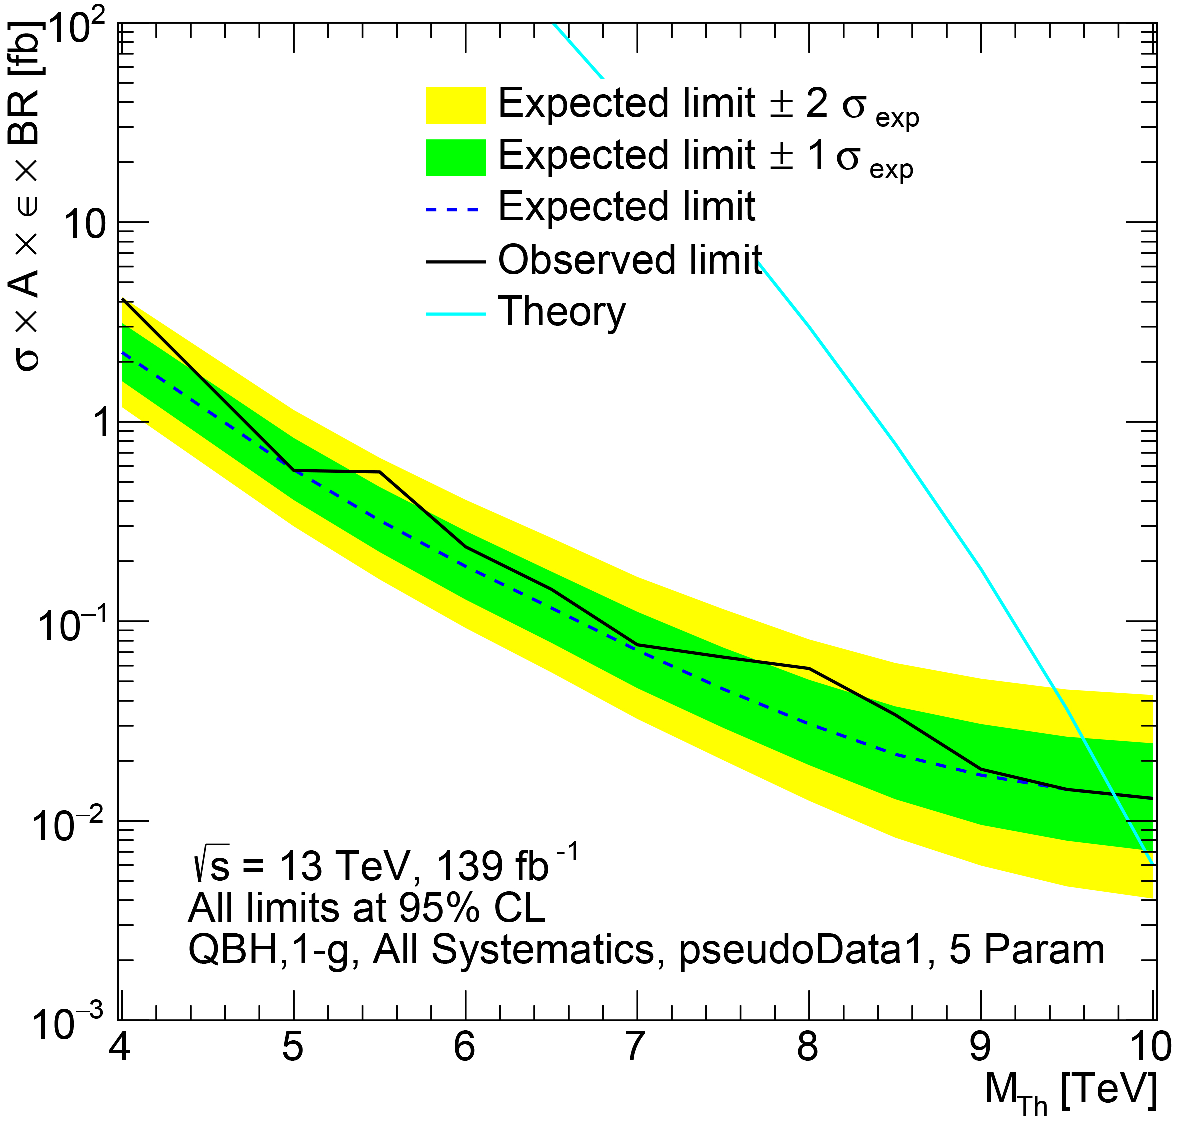
\includegraphics[width=0.45\textwidth]{fig/new_Limit/QBH_Tag1_yStar0p8_data0_Set1_Param5_LumiSyst0p0083_JESJERtrue_sigma.pdf}
  	}\\
  	\subfloat[]{ 
  		%                \label{fig:SignalIndependentGaussianLimits_SubWidth5} % uncomment if label used. 
  		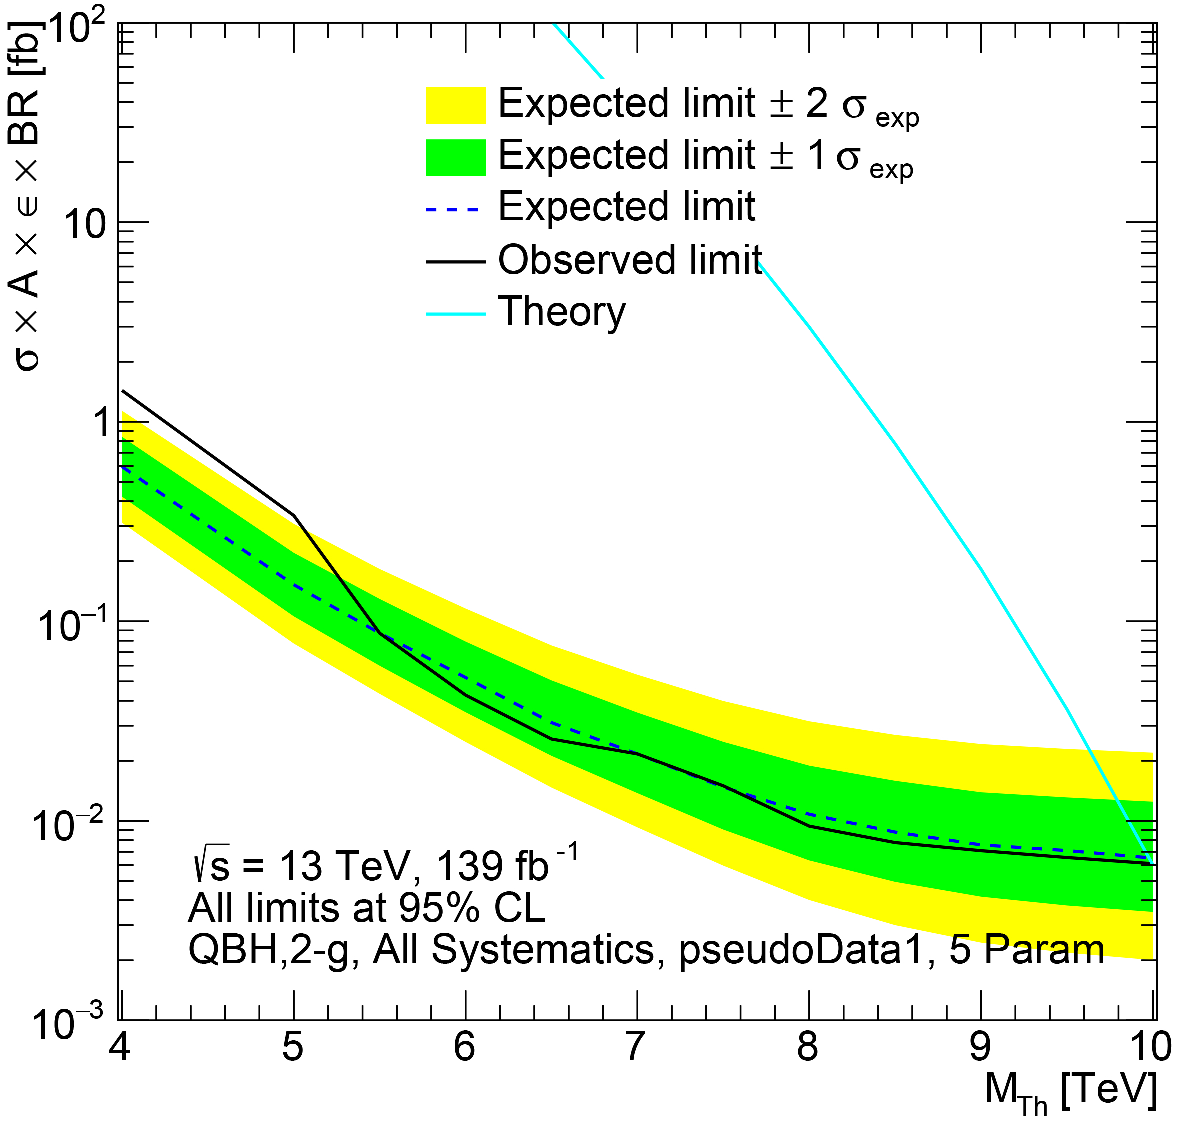
\includegraphics[width=0.45\textwidth]{fig/new_Limit/QBH_Tag2_yStar0p8_data0_Set1_Param5_LumiSyst0p0083_JESJERtrue_sigma.pdf}
  	}
  	\caption{Upper limits set in the untagged (a),  1-$g$ tagged (b) and 2-$g$ (c) tagged Signal Region using QBH model with systematics included using the full 139 fb$^{-1}$ Run-2 dataset.}
  	\label{fig:SignalIndependentGaussianLimits_UntaggedYStar0p81}
  \end{figure}
  

\begin{table}
	\begin{center} 
		\begin{tabular}{ c c c c c c c }
			\hline
			\multicolumn{7}{c}{ untagged  Limits [TeV]}  \\ \hline
			& Obs & Exp $^{+2\sigma}$&Exp $^{+1\sigma}$ &Exp & Exp $^{-1\sigma}$&Exp $^{-2\sigma}$\\	\hline
			Graviton&3.78 &3.15&3.35  &3.60 &3.80&4.11\\\hline
			QBH&9.57 &9.19&9.56 &9.76 &9.98&10.01\\
			\hline
		\end{tabular}
		\caption{ Limits in the untagged region for signal models.}
		\label{tab:0g}
	\end{center}
\end{table}

\begin{table}
\begin{center} 
\begin{tabular}{ c c c c c c c }
	\hline
	\multicolumn{7}{c}{ 1-$g$ tagged  Limits [TeV]}  \\ \hline
	 & Obs & Exp $^{+2\sigma}$&Exp $^{+1\sigma}$ &Exp & Exp $^{-1\sigma}$&Exp $^{-2\sigma}$\\	\hline
	Graviton&4.01 &3.36&3.51  &3.85 &4.00&4.31\\\hline
QBH&9.88 &9.47&9.68 &9.88 &9.99&10.04\\
	\hline
\end{tabular}
		\caption{ Limits in the 1-$g$ tagged region for signal models.}
\label{tab:1g}
	\end{center}
\end{table}

\begin{table}
\begin{center}
\begin{tabular}{ c c c c c c c }
	\hline
	\multicolumn{7}{c}{ 2-$g$ tagged  Limits [TeV]}  \\ \hline
	& Obs & Exp $^{+2\sigma}$&Exp $^{+1\sigma}$ &Exp & Exp $^{-1\sigma}$&Exp $^{-2\sigma}$\\	\hline
	Graviton&4.26&3.93&4.15 &4.41&4.66&4.93\\\hline
	QBH&10.00 &9.73&9.90 &10.00  &10.05&10.07\\
	\hline
\end{tabular}
	\caption{Limits in the 2-$g$ tagged region for signal models.}
\label{tab:2g}
	\end{center}
\end{table}


%model-independent Gaussian limits are shown in fig \ref{fig:SignalIndependentGaussianLimits_UntaggedYStar0p8}, \ref{fig:SignalIndependentGaussianLimits_1gYStar0p6} and \ref{fig:SignalIndependentGaussianLimits_2gYStar0p8} respectively, for Gaussians with width equal to 0, 3, 5, 7, 10 and 15\% of their peak position, without systematics included. 

%        \begin{figure}[!htb]
%            \subfloat[0\% Width Gaussian Limits]{ 
%%                \label{fig:SignalIndependentGaussianLimits_SubWidth0} % uncomment if label used. 
%                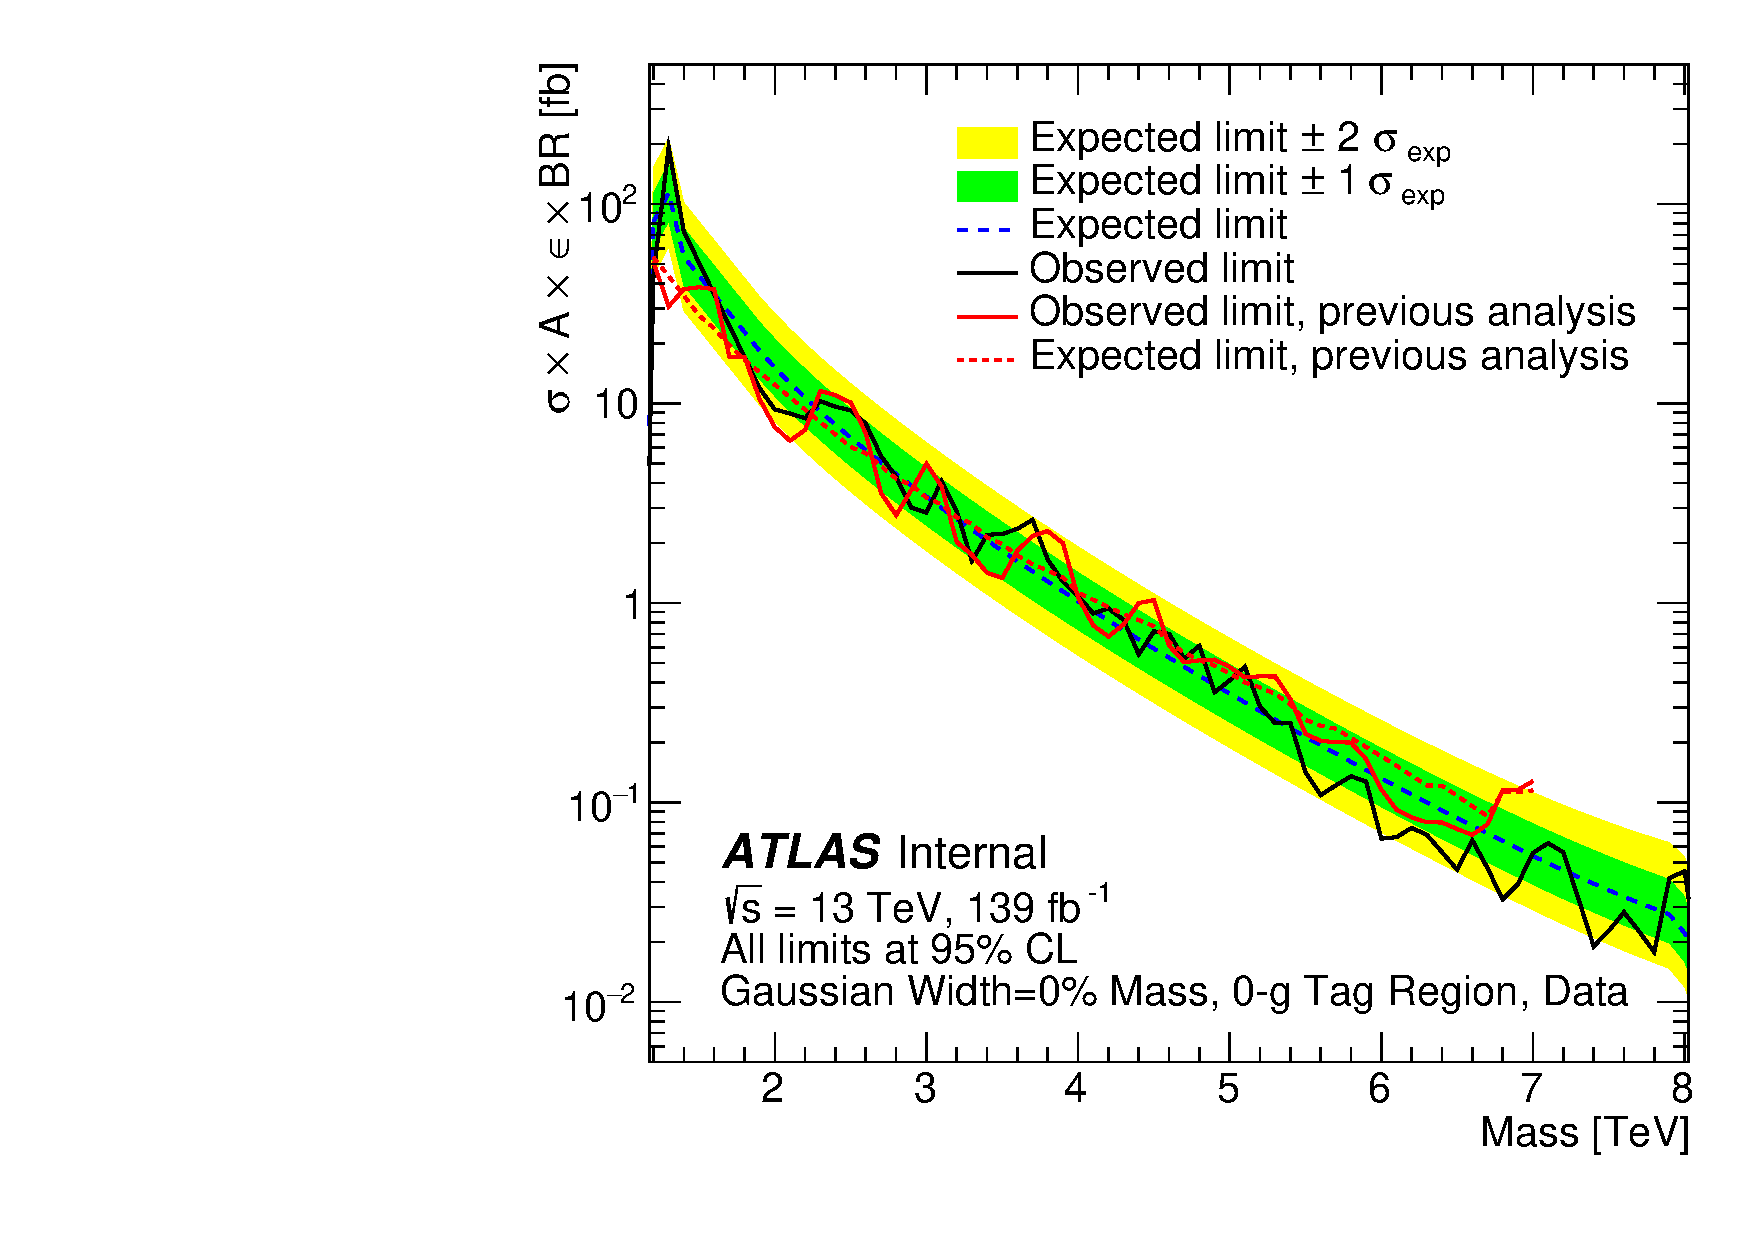
\includegraphics[width=0.4\textwidth]{fig/app-SignalIndependentLimits/Gauss_Limits_yStar0p8_Tag0_WidthPercent0_1200to8000_sigma.pdf}
%            }
%            \subfloat[3\% Width Gaussian Limits]{ 
%%                \label{fig:SignalIndependentGaussianLimits_SubWidth3} % uncomment if label used. 
%                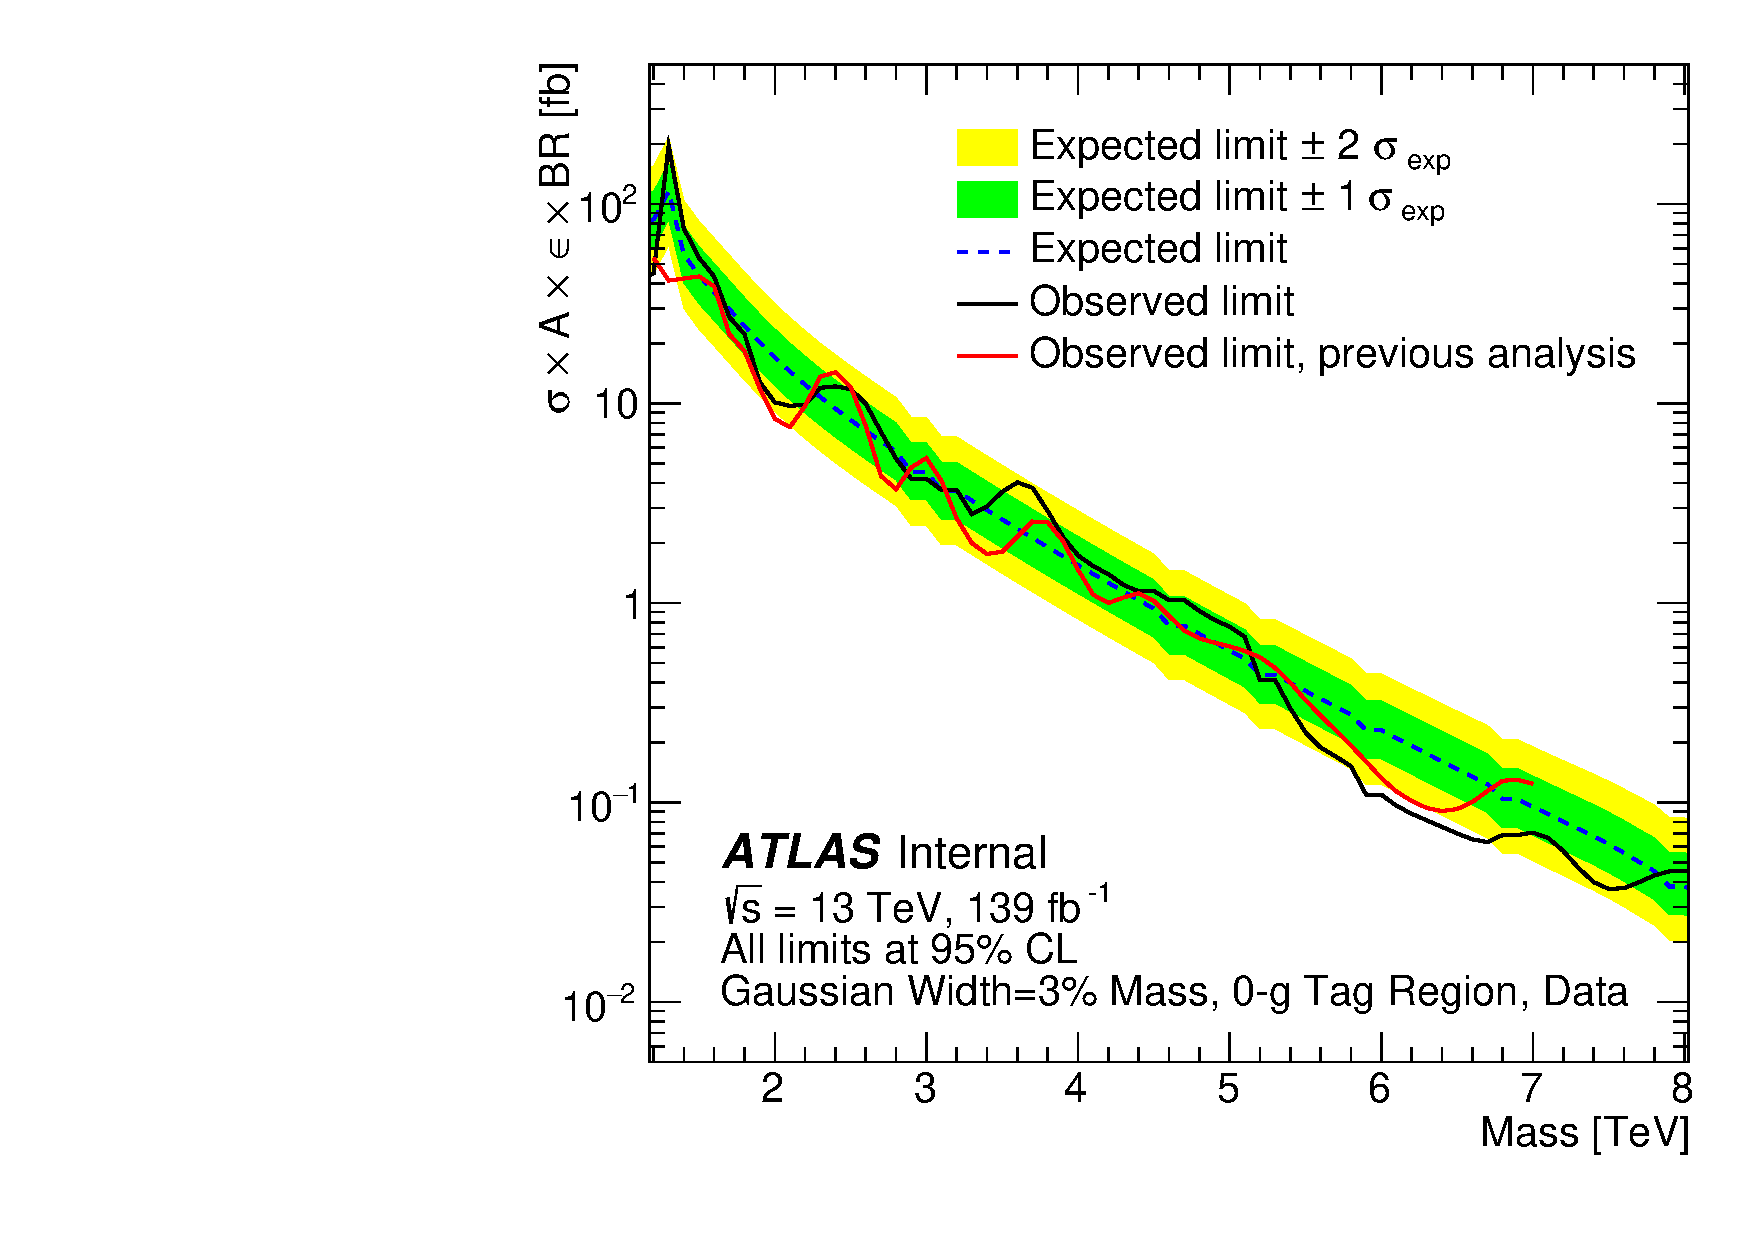
\includegraphics[width=0.4\textwidth]{fig/app-SignalIndependentLimits/Gauss_Limits_yStar0p8_Tag0_WidthPercent3_1200to8000_sigma.pdf}
%            }\\
%            \subfloat[5\% Width Gaussian Limits]{ 
%%                \label{fig:SignalIndependentGaussianLimits_SubWidth5} % uncomment if label used. 
%                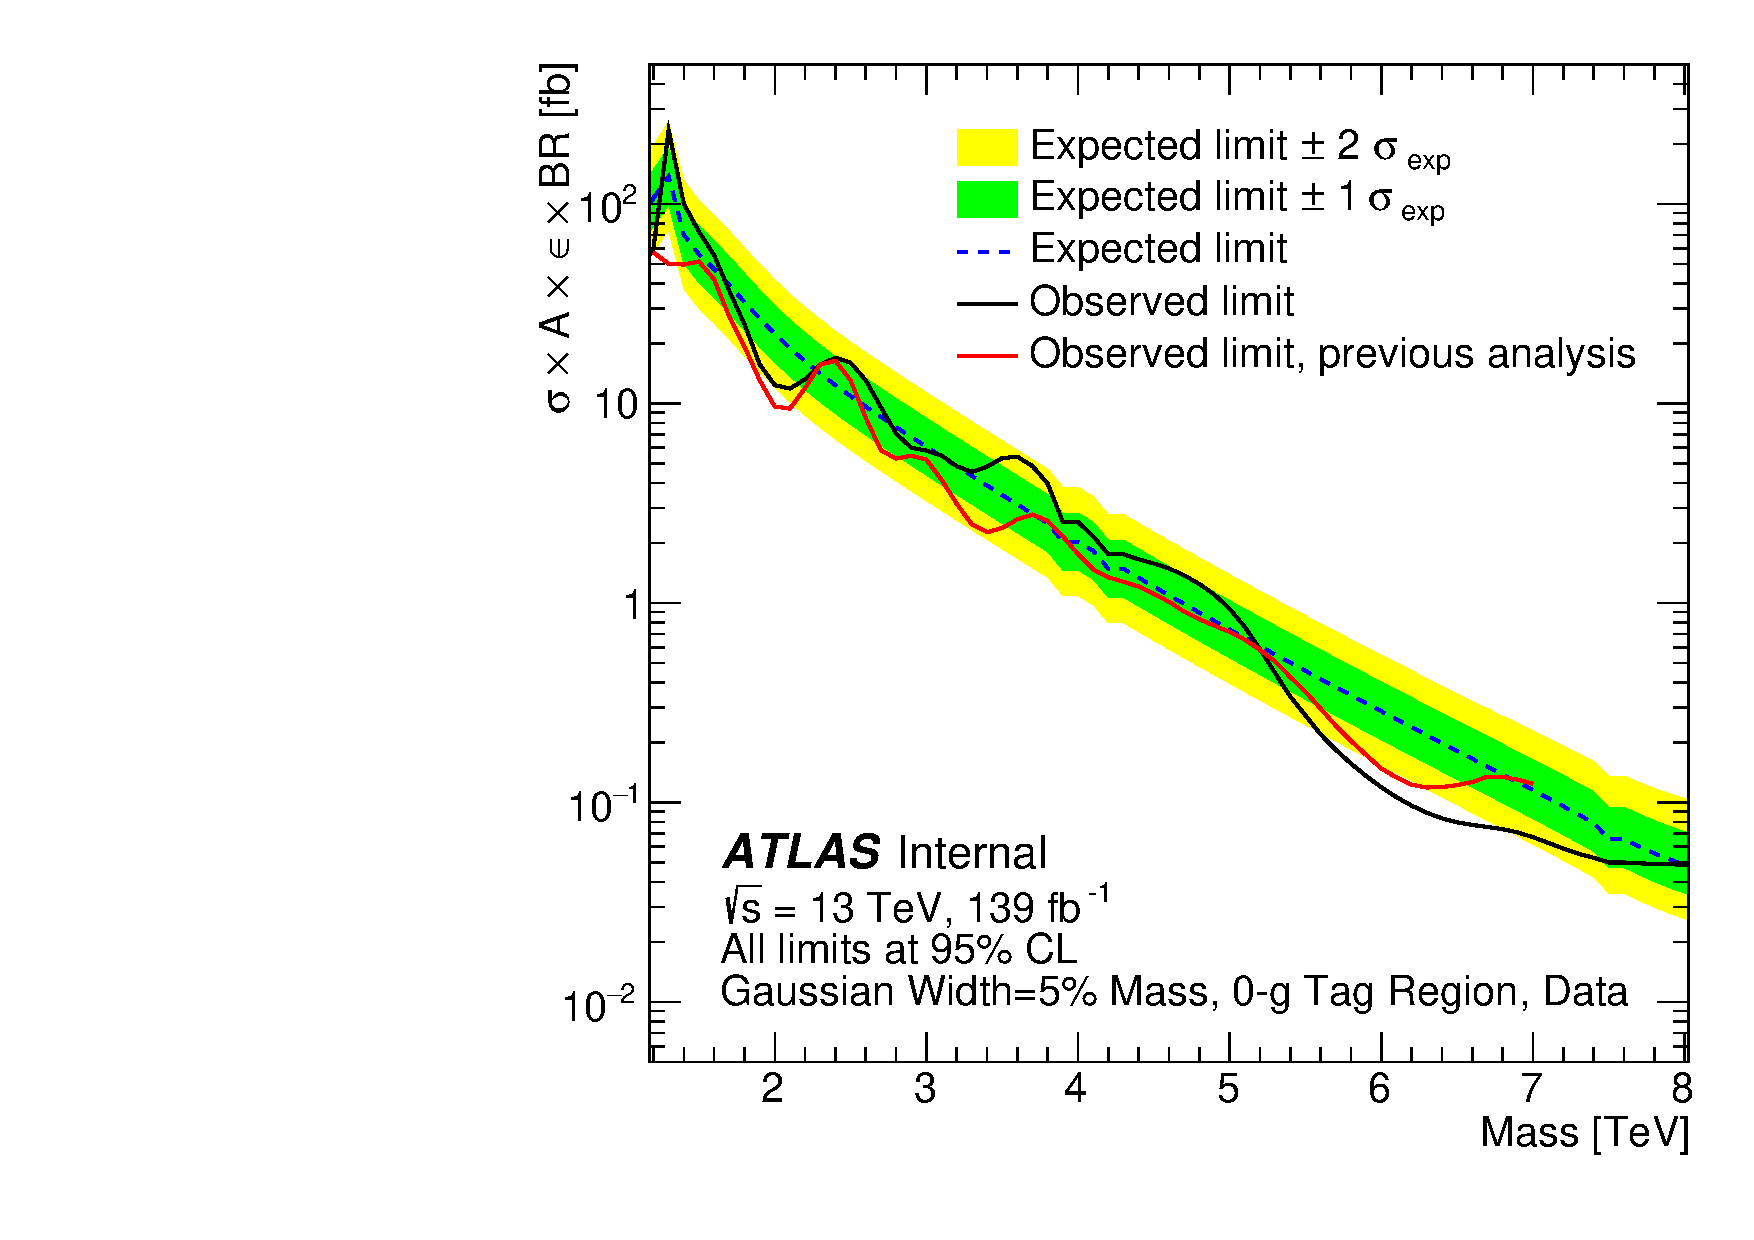
\includegraphics[width=0.4\textwidth]{fig/app-SignalIndependentLimits/Gauss_Limits_yStar0p8_Tag0_WidthPercent5_1200to8000_sigma.pdf}
%            }
%            \subfloat[7\% Width Gaussian Limits]{ 
%%                \label{fig:SignalIndependentGaussianLimits_SubWidth7} % uncomment if label used. 
%                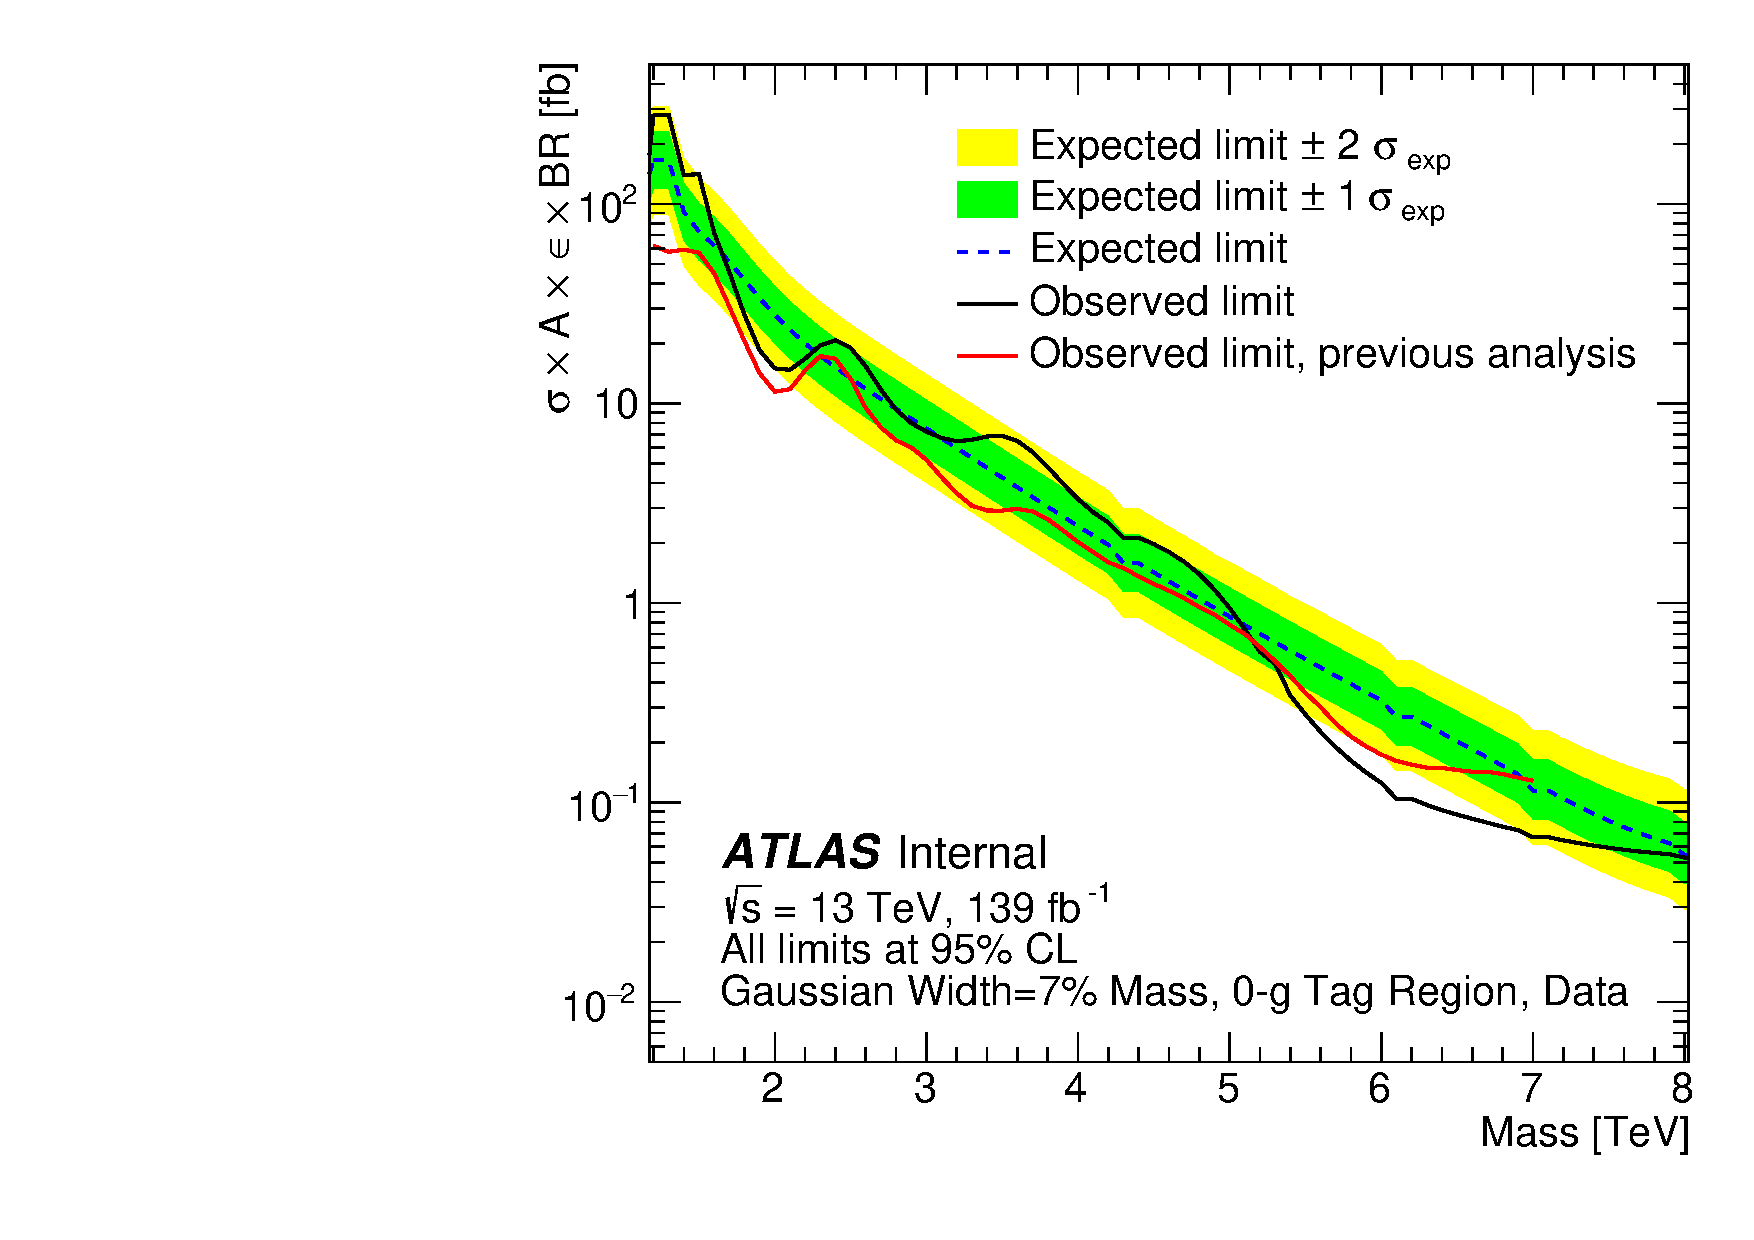
\includegraphics[width=0.4\textwidth]{fig/app-SignalIndependentLimits/Gauss_Limits_yStar0p8_Tag0_WidthPercent7_1200to8000_sigma.pdf}
%            }\\
%            \subfloat[10\% Width Gaussian Limits]{ 
%%                \label{fig:SignalIndependentGaussianLimits_SubWidth10} % uncomment if label used. 
%                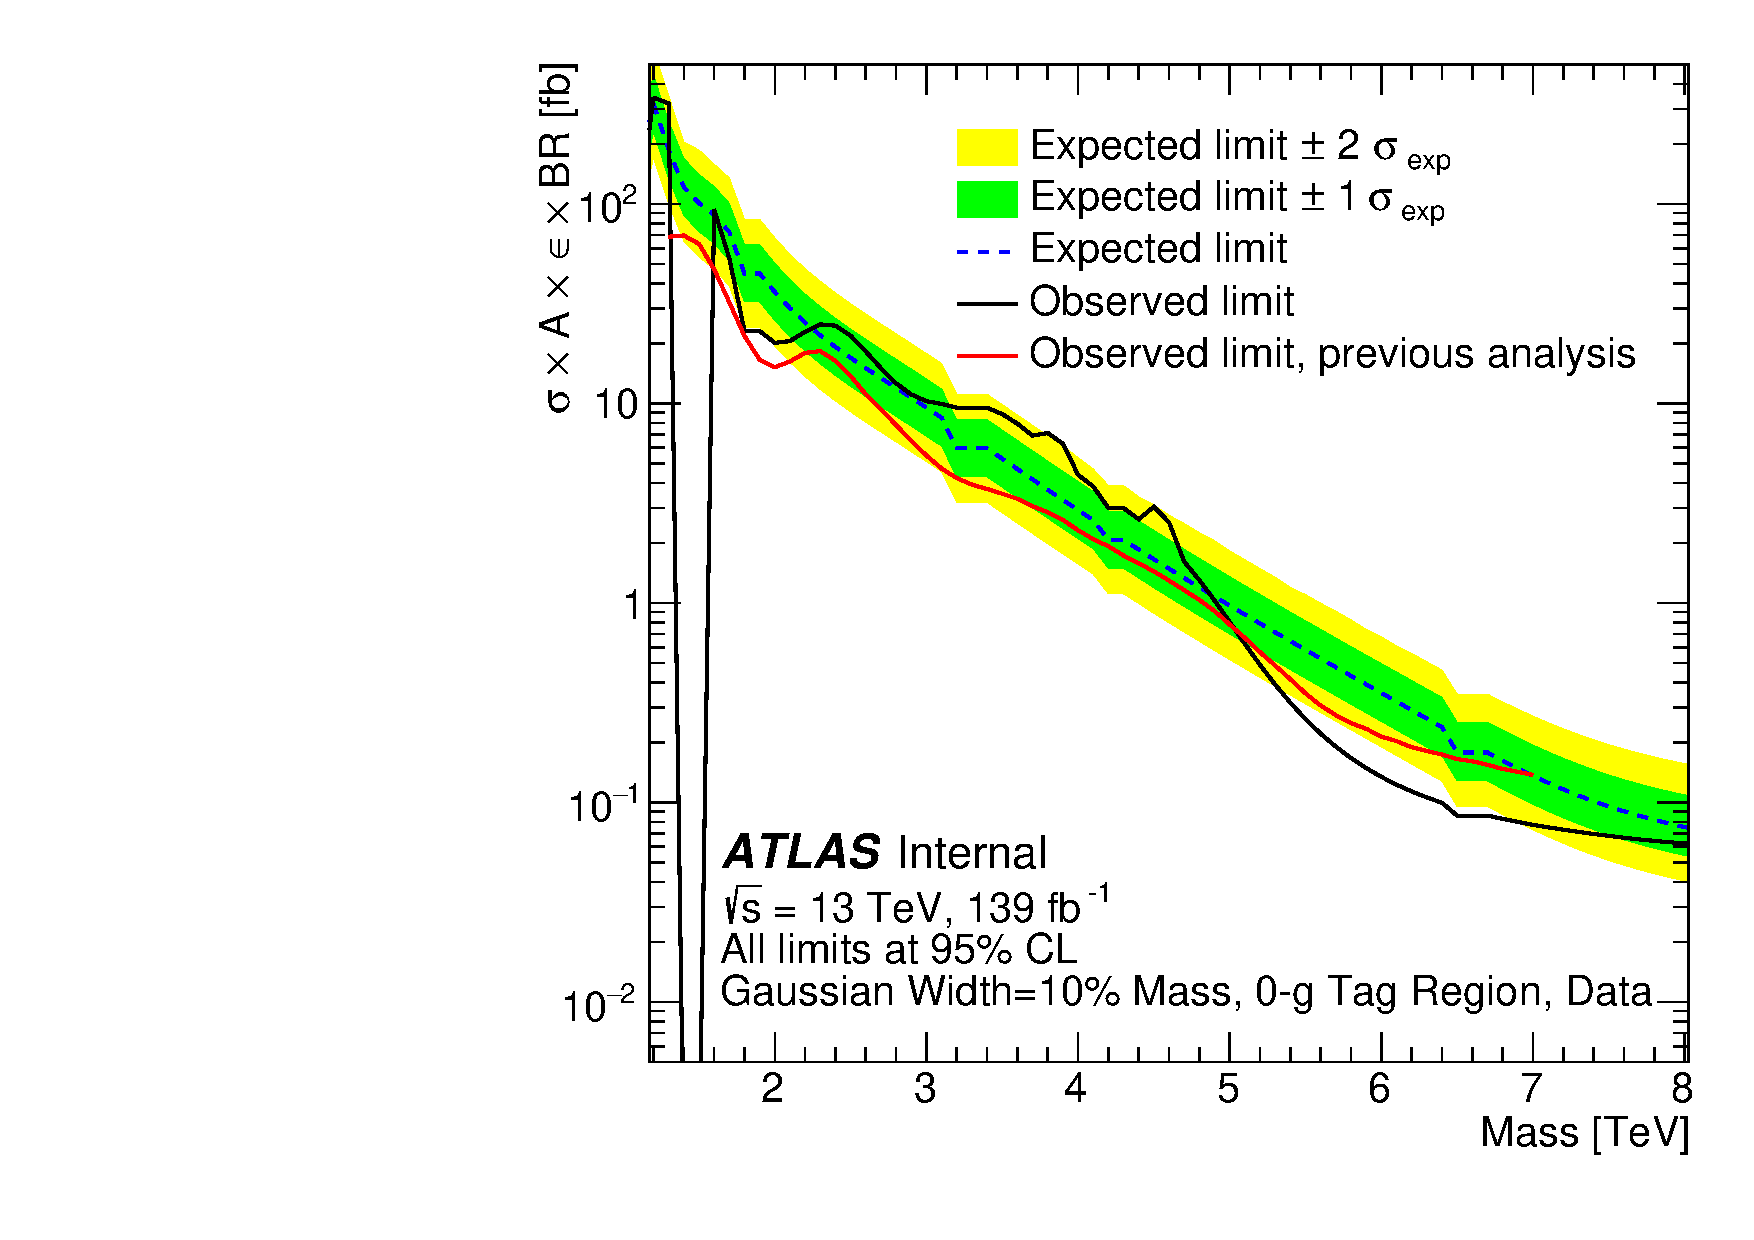
\includegraphics[width=0.4\textwidth]{fig/app-SignalIndependentLimits/Gauss_Limits_yStar0p8_Tag0_WidthPercent10_1200to8000_sigma.pdf}
%            }
%            \subfloat[15\% Width Gaussian Limits]{ 
%%                \label{fig:SignalIndependentGaussianLimits_SubWidth15} % uncomment if label used. 
%                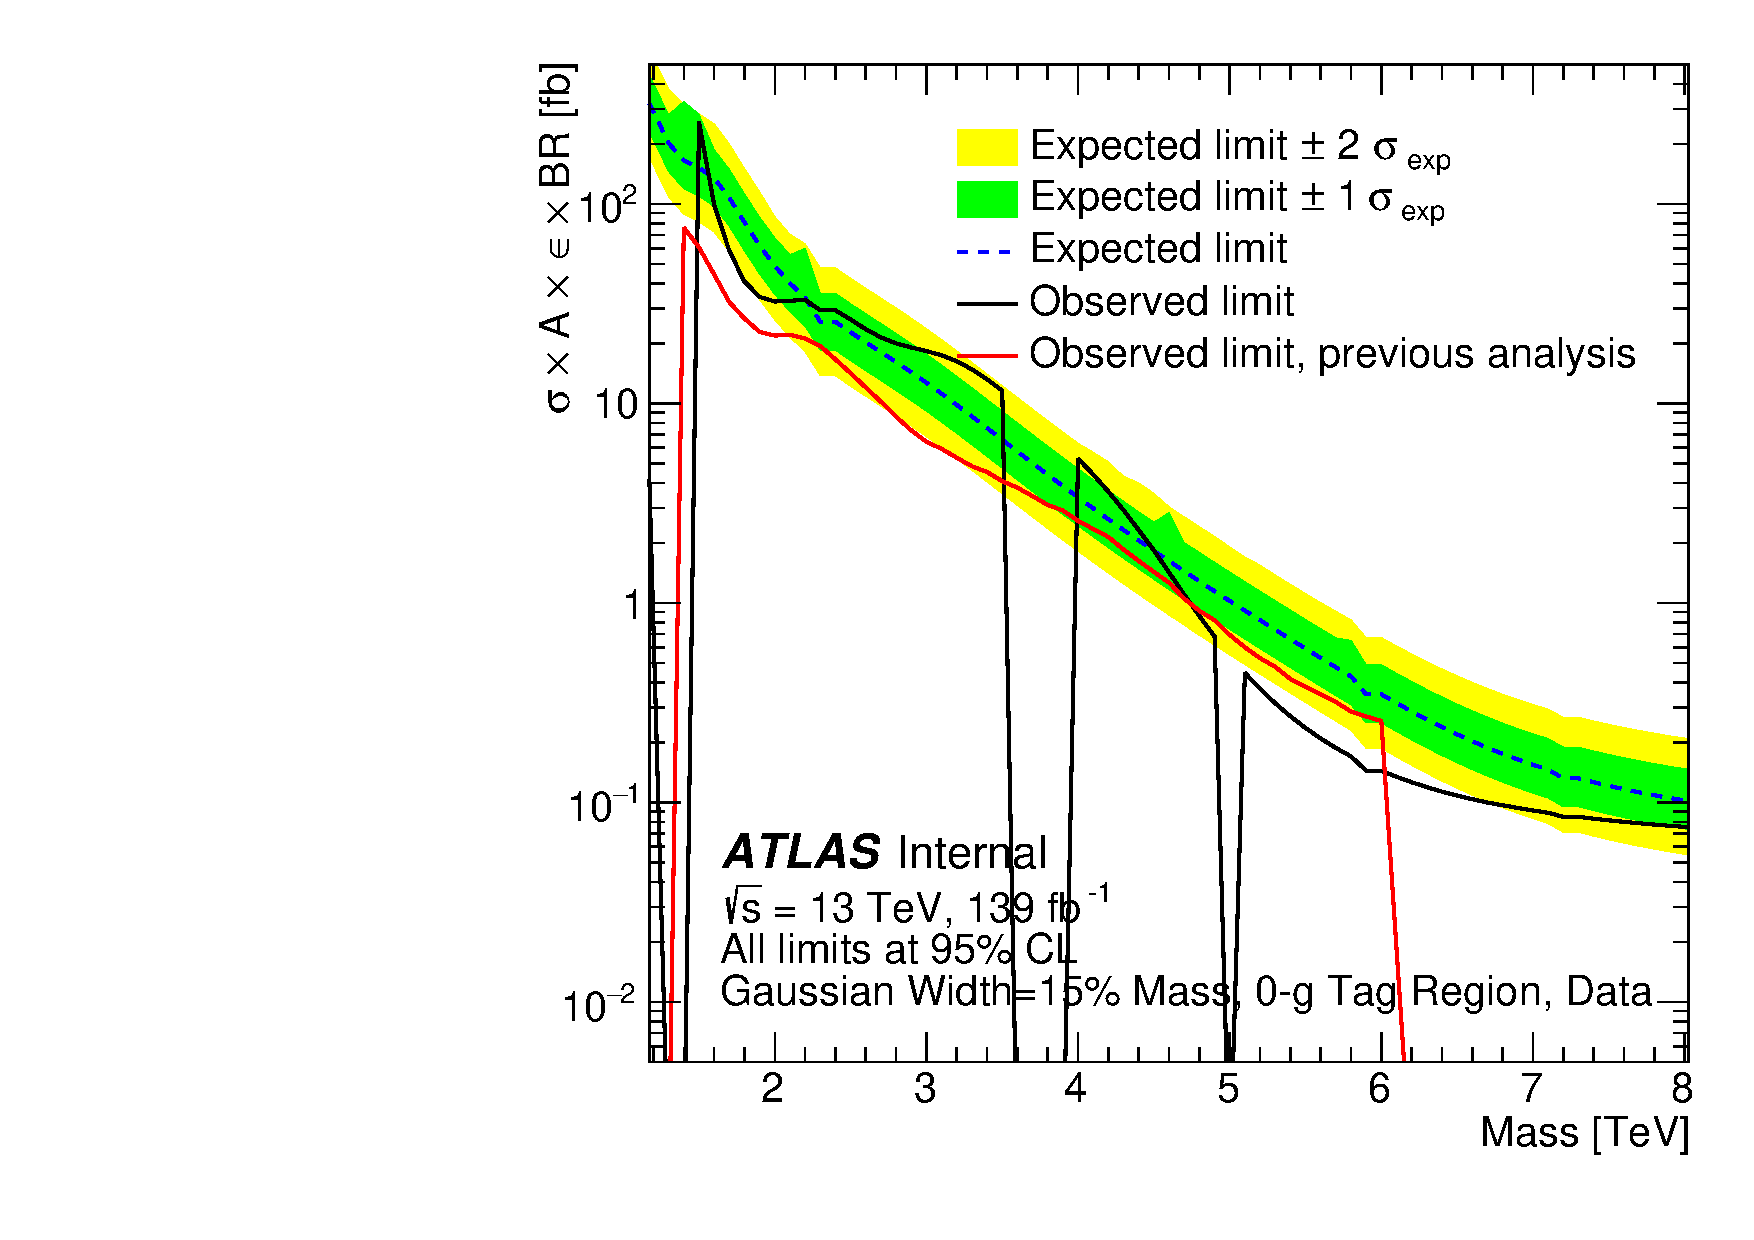
\includegraphics[width=0.4\textwidth]{fig/app-SignalIndependentLimits/Gauss_Limits_yStar0p8_Tag0_WidthPercent15_1200to8000_sigma.pdf}
%            }
%            \caption{Model-independent limits set in the untagged $y^{*} < 0.8$ Signal Region using Gaussian resonances of varying widths from 0\% to 15\% of their peak position without systematics included using the full 139fb$^{-1}$ Run-2 dataset.}
%            \label{fig:SignalIndependentGaussianLimits_UntaggedYStar0p8}
%        \end{figure}
%
%
%        \begin{figure}[!htb]
%            \subfloat[0\% Width Gaussian Limits]{ 
%%                \label{fig:SignalIndependentGaussianLimits_SubWidth0} % uncomment if label used. 
%                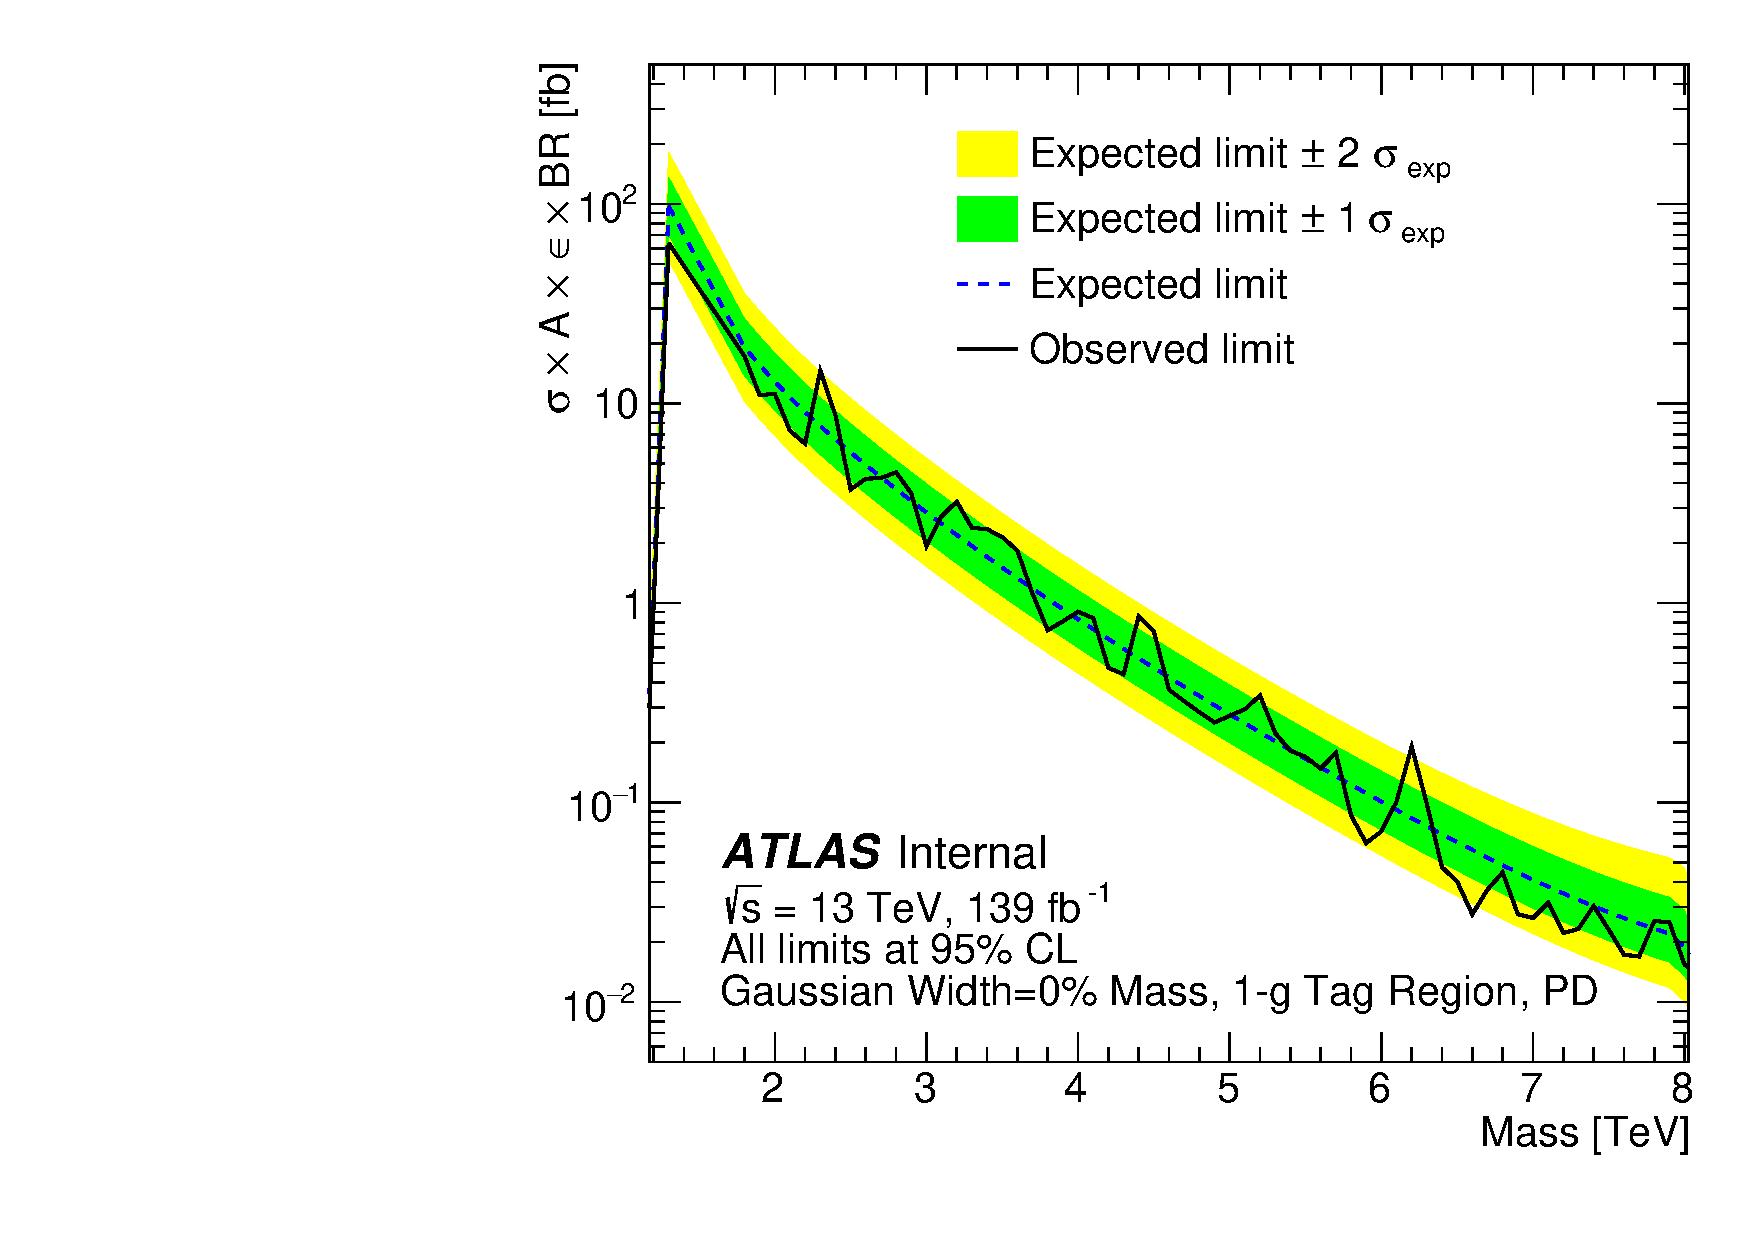
\includegraphics[width=0.4\textwidth]{fig/app-SignalIndependentLimits/Gauss_Limits_yStar0p6_Tag1_WidthPercent0_1200to8000_sigma.pdf}
%            }
%            \subfloat[3\% Width Gaussian Limits]{ 
%%                \label{fig:SignalIndependentGaussianLimits_SubWidth3} % uncomment if label used. 
%                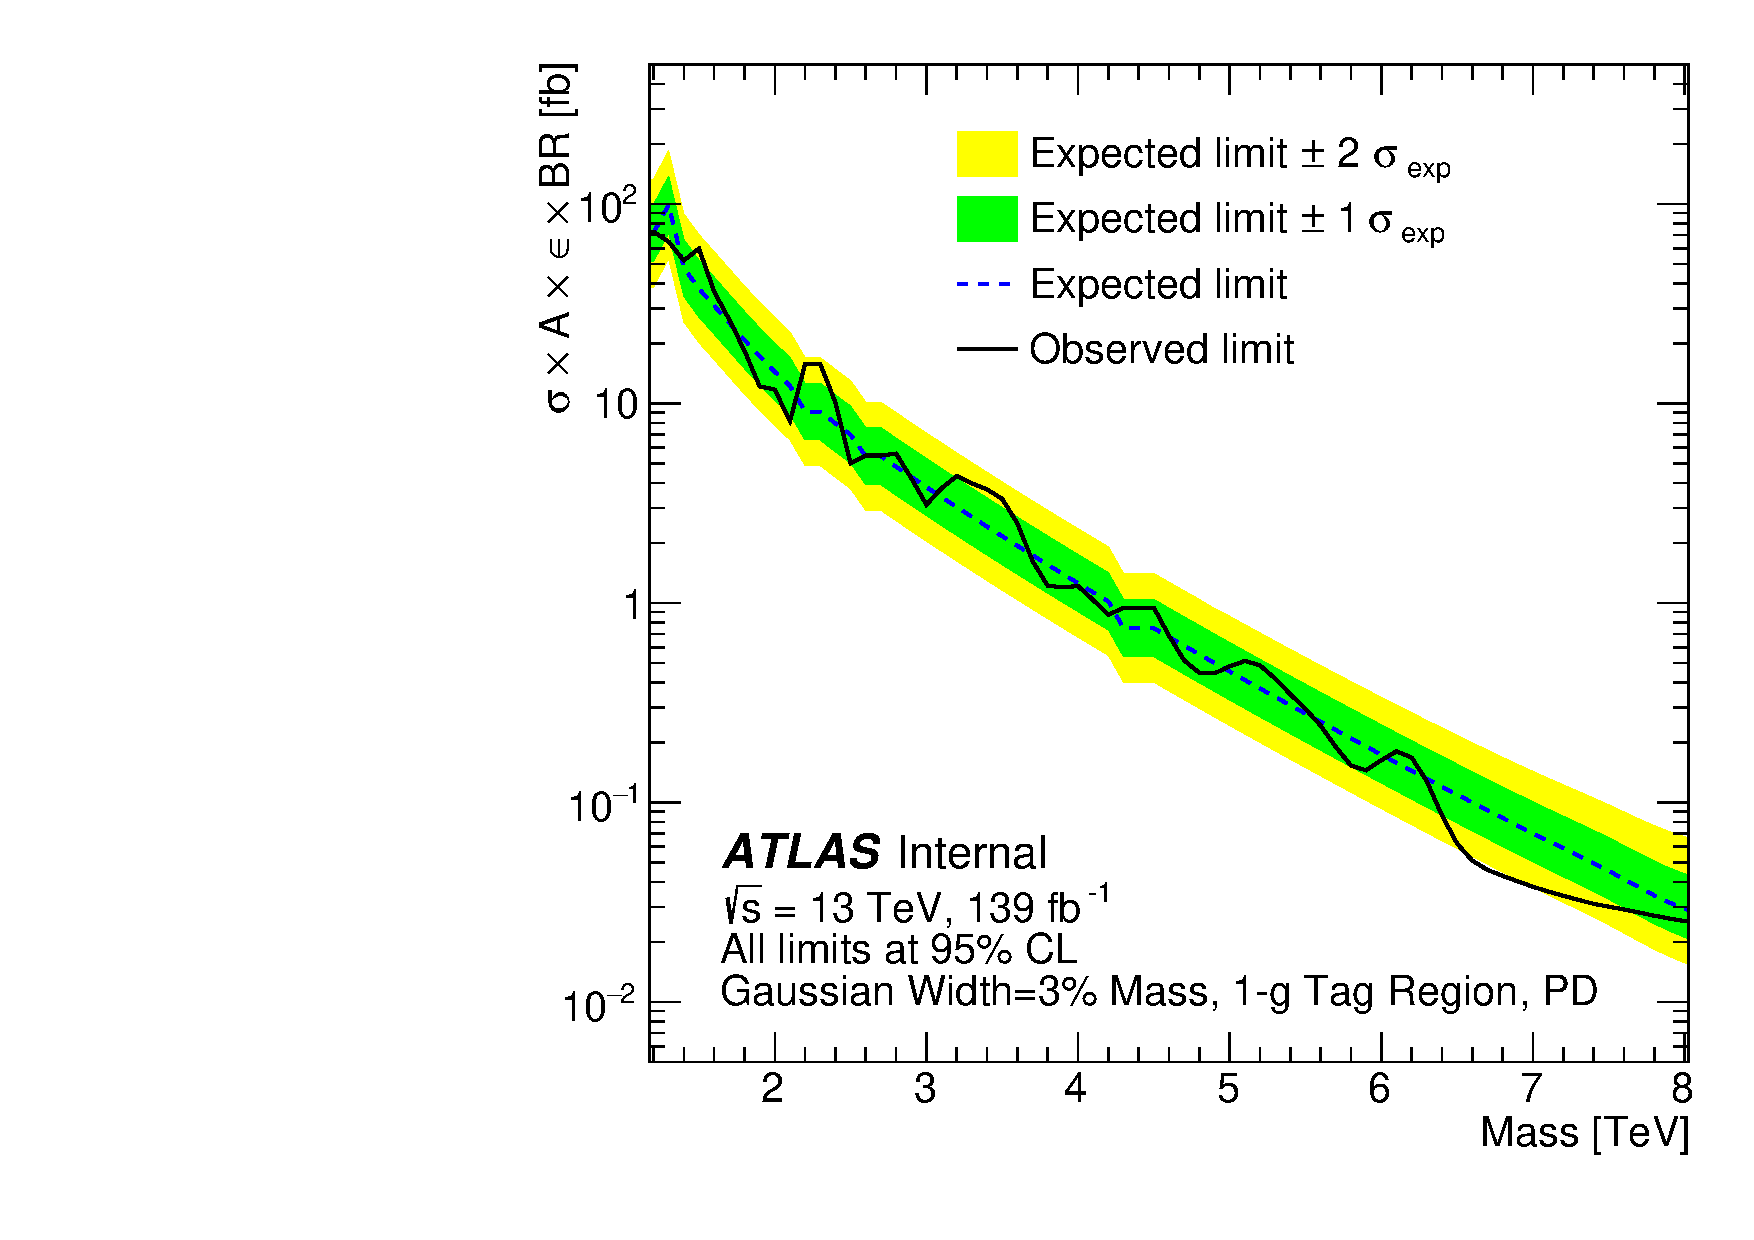
\includegraphics[width=0.4\textwidth]{fig/app-SignalIndependentLimits/Gauss_Limits_yStar0p6_Tag1_WidthPercent3_1200to8000_sigma.pdf}
%            }\\
%            \subfloat[5\% Width Gaussian Limits]{ 
%%                \label{fig:SignalIndependentGaussianLimits_SubWidth5} % uncomment if label used. 
%                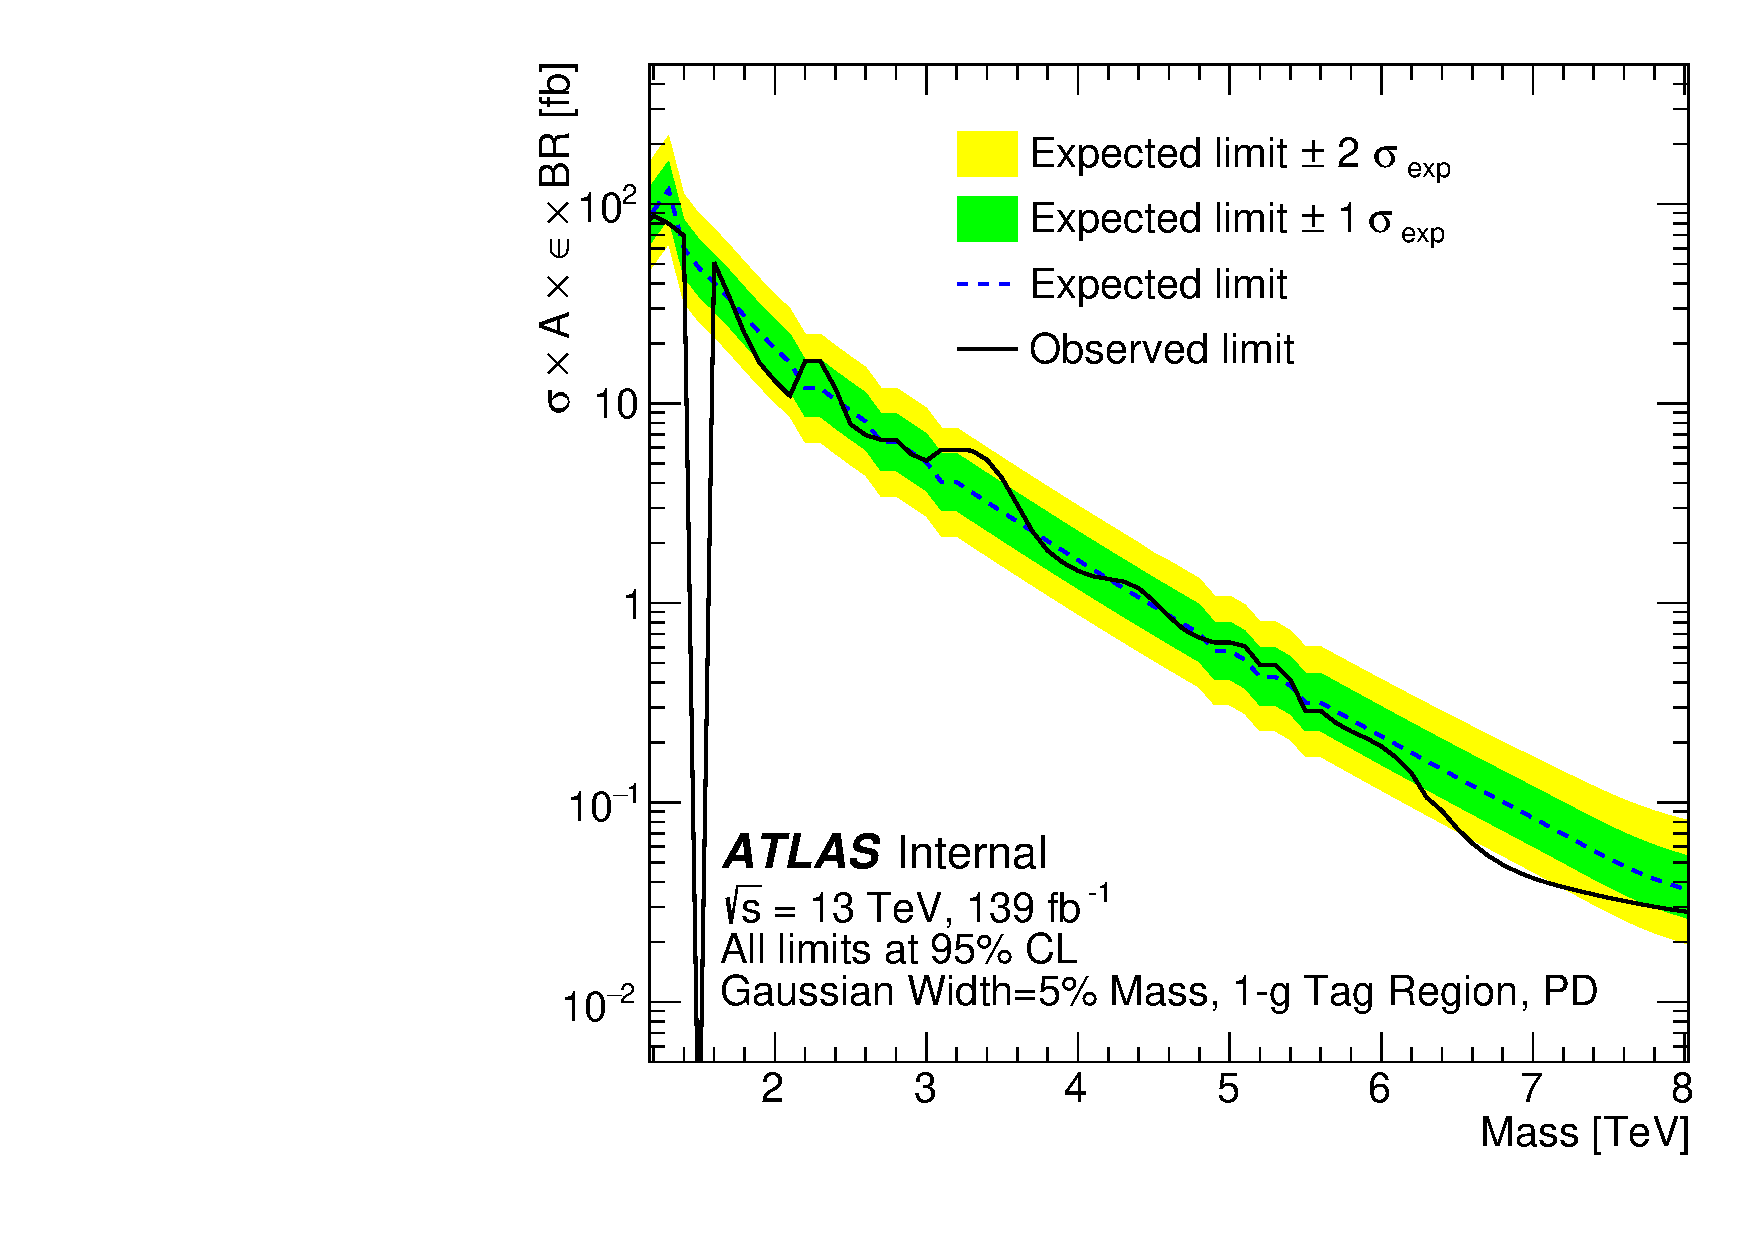
\includegraphics[width=0.4\textwidth]{fig/app-SignalIndependentLimits/Gauss_Limits_yStar0p6_Tag1_WidthPercent5_1200to8000_sigma.pdf}
%            }
%            \subfloat[7\% Width Gaussian Limits]{ 
%%                \label{fig:SignalIndependentGaussianLimits_SubWidth7} % uncomment if label used. 
%                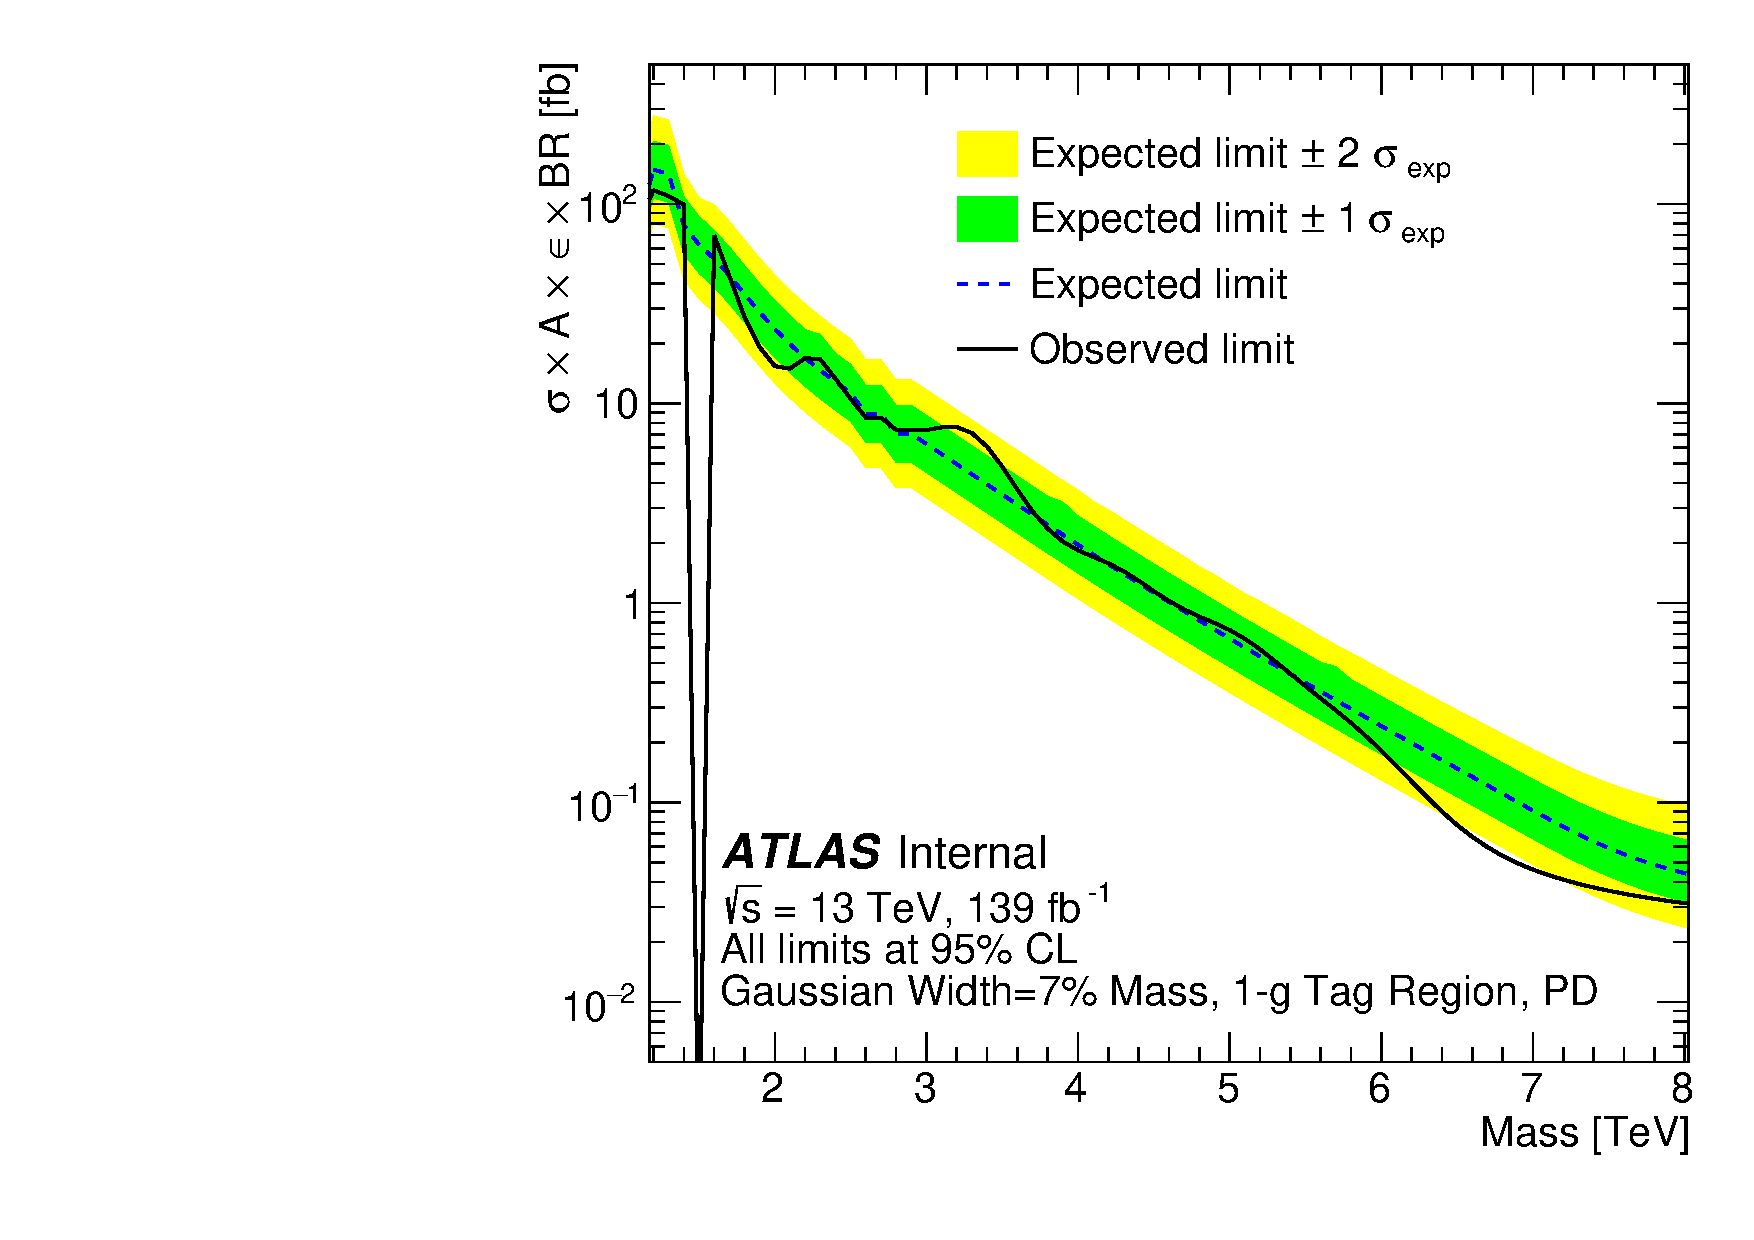
\includegraphics[width=0.4\textwidth]{fig/app-SignalIndependentLimits/Gauss_Limits_yStar0p6_Tag1_WidthPercent7_1200to8000_sigma.pdf}
%            }\\
%            \subfloat[10\% Width Gaussian Limits]{ 
%%                \label{fig:SignalIndependentGaussianLimits_SubWidth10} % uncomment if label used. 
%                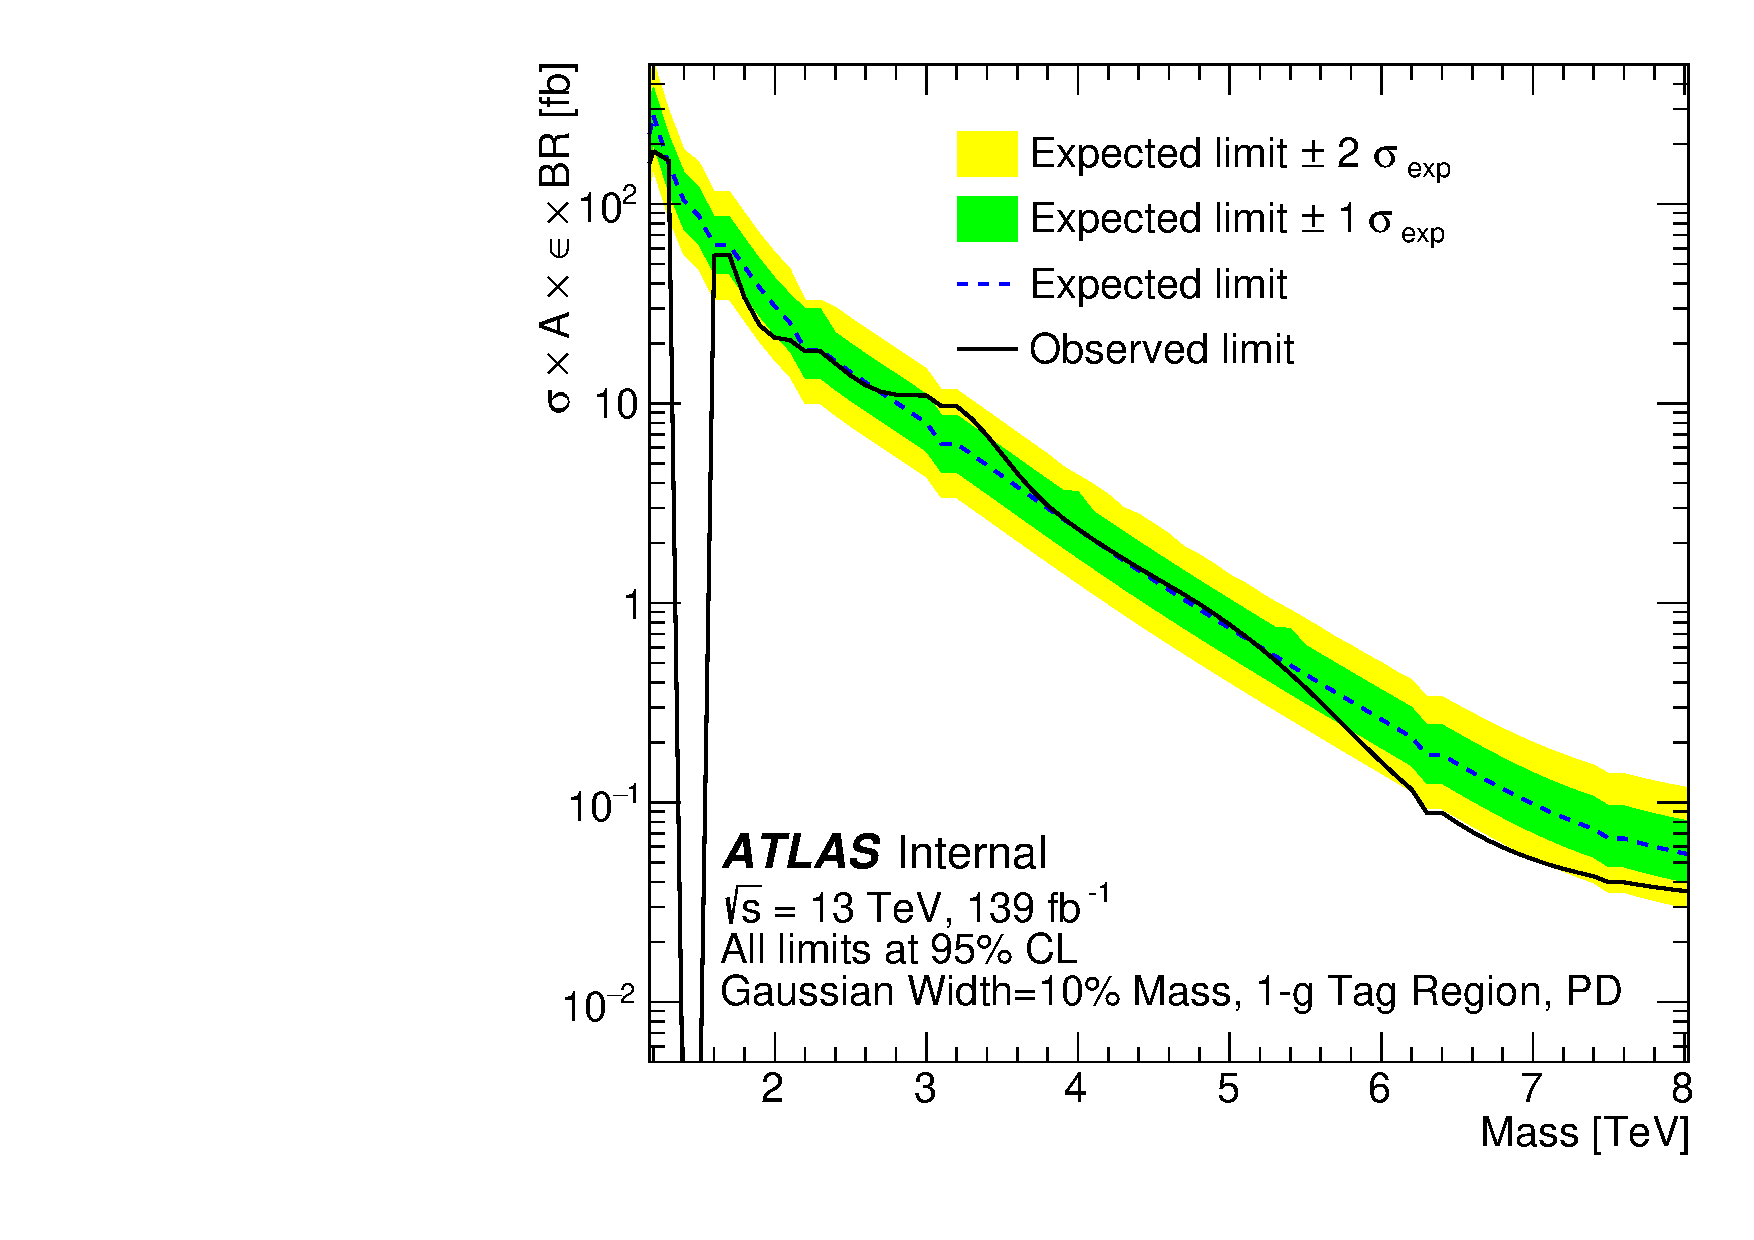
\includegraphics[width=0.4\textwidth]{fig/app-SignalIndependentLimits/Gauss_Limits_yStar0p6_Tag1_WidthPercent10_1200to8000_sigma.pdf}
%            }
%            \subfloat[15\% Width Gaussian Limits]{ 
%%                \label{fig:SignalIndependentGaussianLimits_SubWidth15} % uncomment if label used. 
%                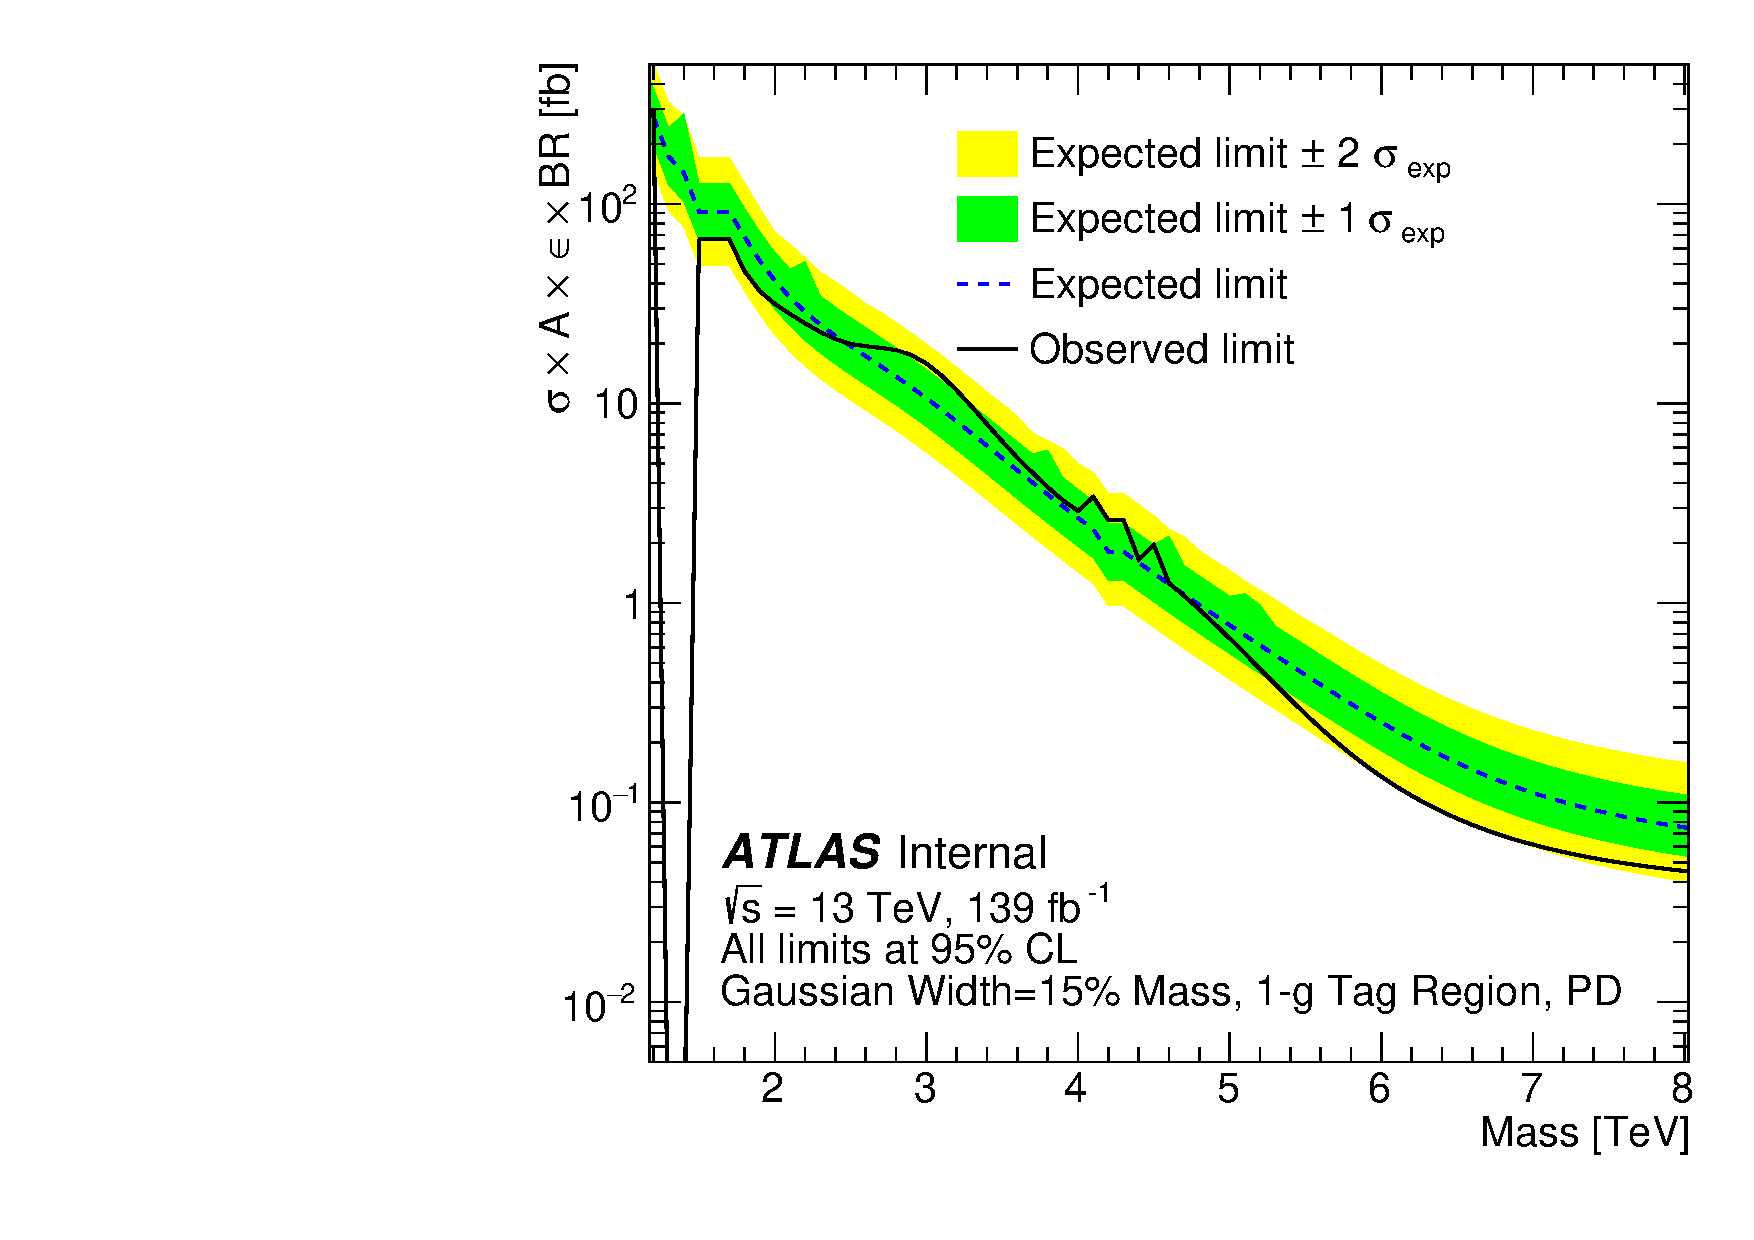
\includegraphics[width=0.4\textwidth]{fig/app-SignalIndependentLimits/Gauss_Limits_yStar0p6_Tag1_WidthPercent15_1200to8000_sigma.pdf}
%            }
%            \caption{Model-independent limits set in the 1-$g$ tagged $y^{*} < 0.6$ Signal Region using Gaussian resonances of varying widths from 0\% to 15\% of their peak position without systematics included using the full 139fb$^{-1}$ Run-2 dataset.}
%            \label{fig:SignalIndependentGaussianLimits_1gYStar0p6}
%        \end{figure}
%
%        \begin{figure}[!htb]
%            \subfloat[0\% Width Gaussian Limits]{ 
%%                \label{fig:SignalIndependentGaussianLimits_SubWidth0} % uncomment if label used. 
%                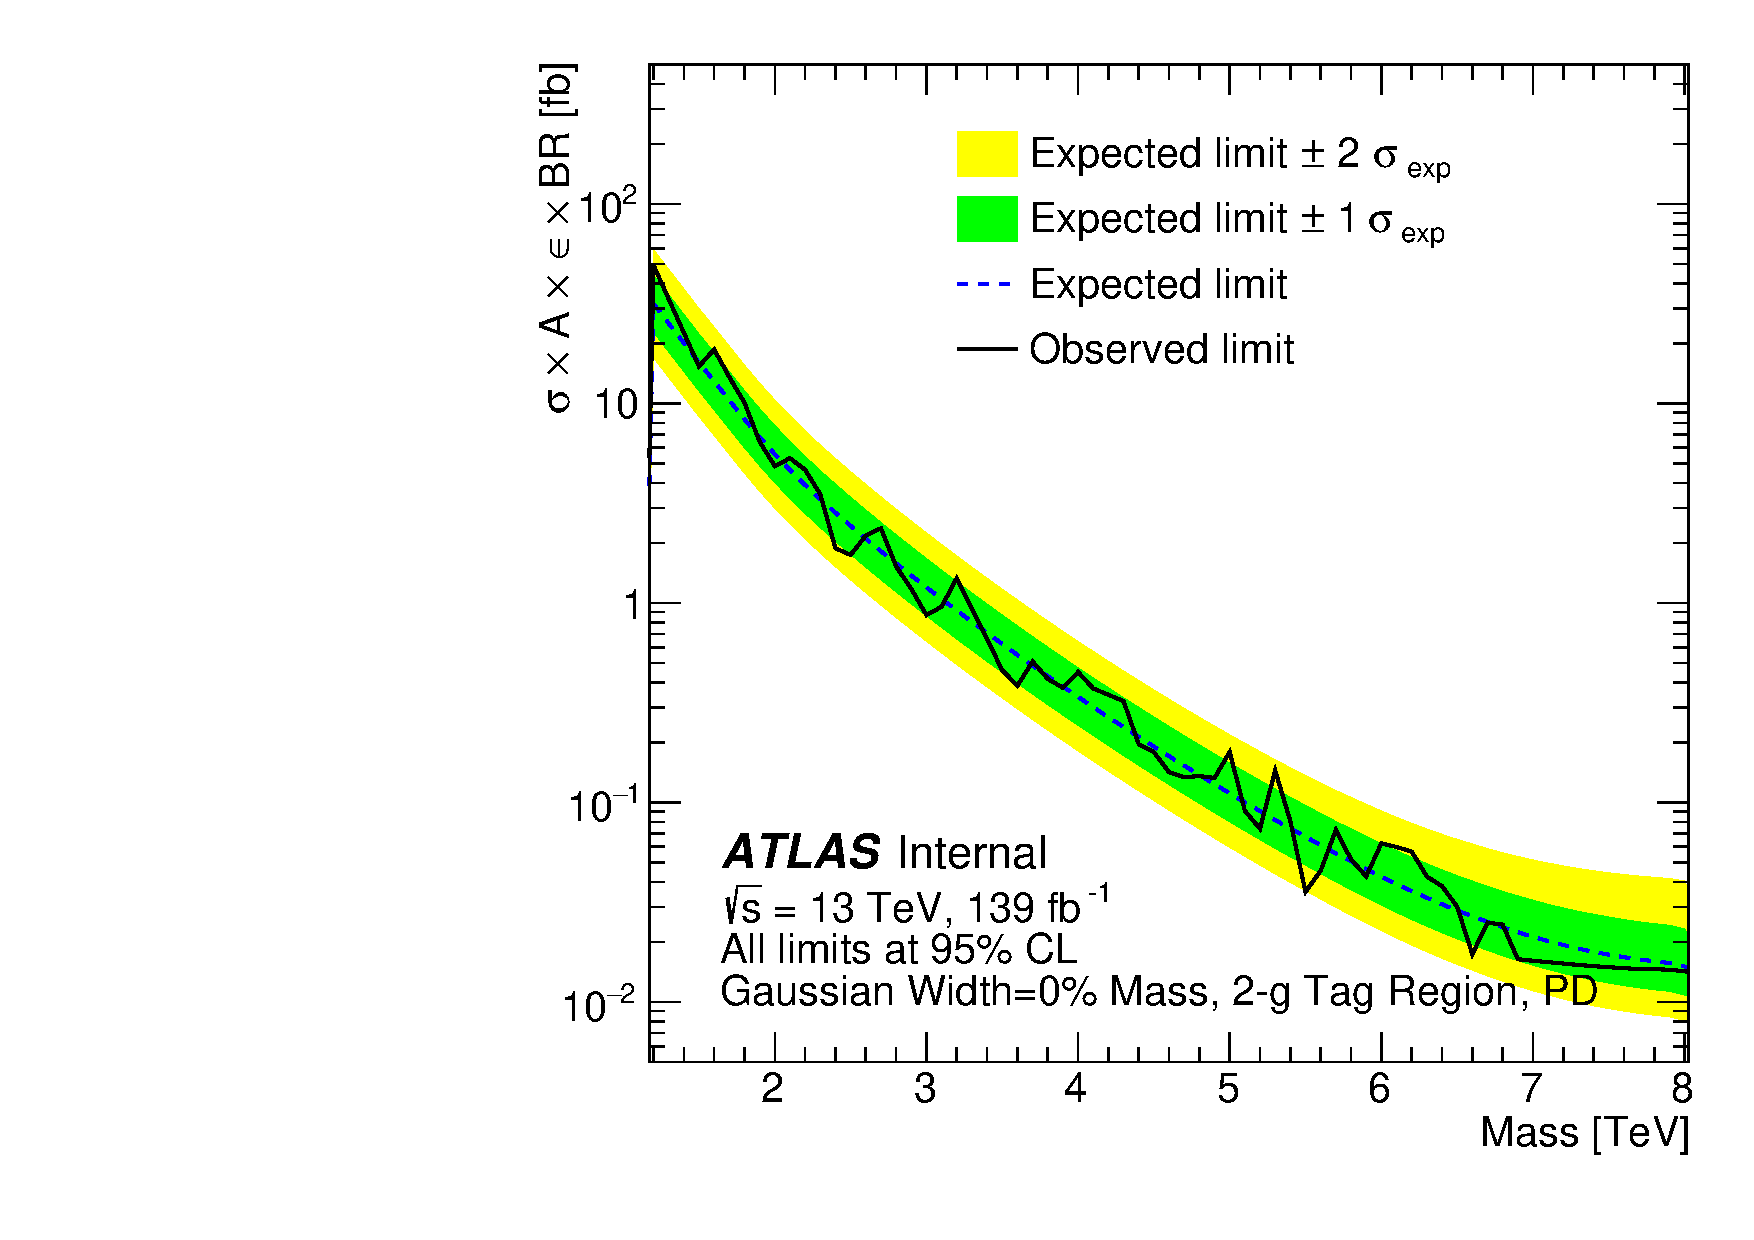
\includegraphics[width=0.4\textwidth]{fig/app-SignalIndependentLimits/Gauss_Limits_yStar0p8_Tag2_WidthPercent0_1200to8000_sigma.pdf}
%            }
%            \subfloat[3\% Width Gaussian Limits]{ 
%%                \label{fig:SignalIndependentGaussianLimits_SubWidth3} % uncomment if label used. 
%                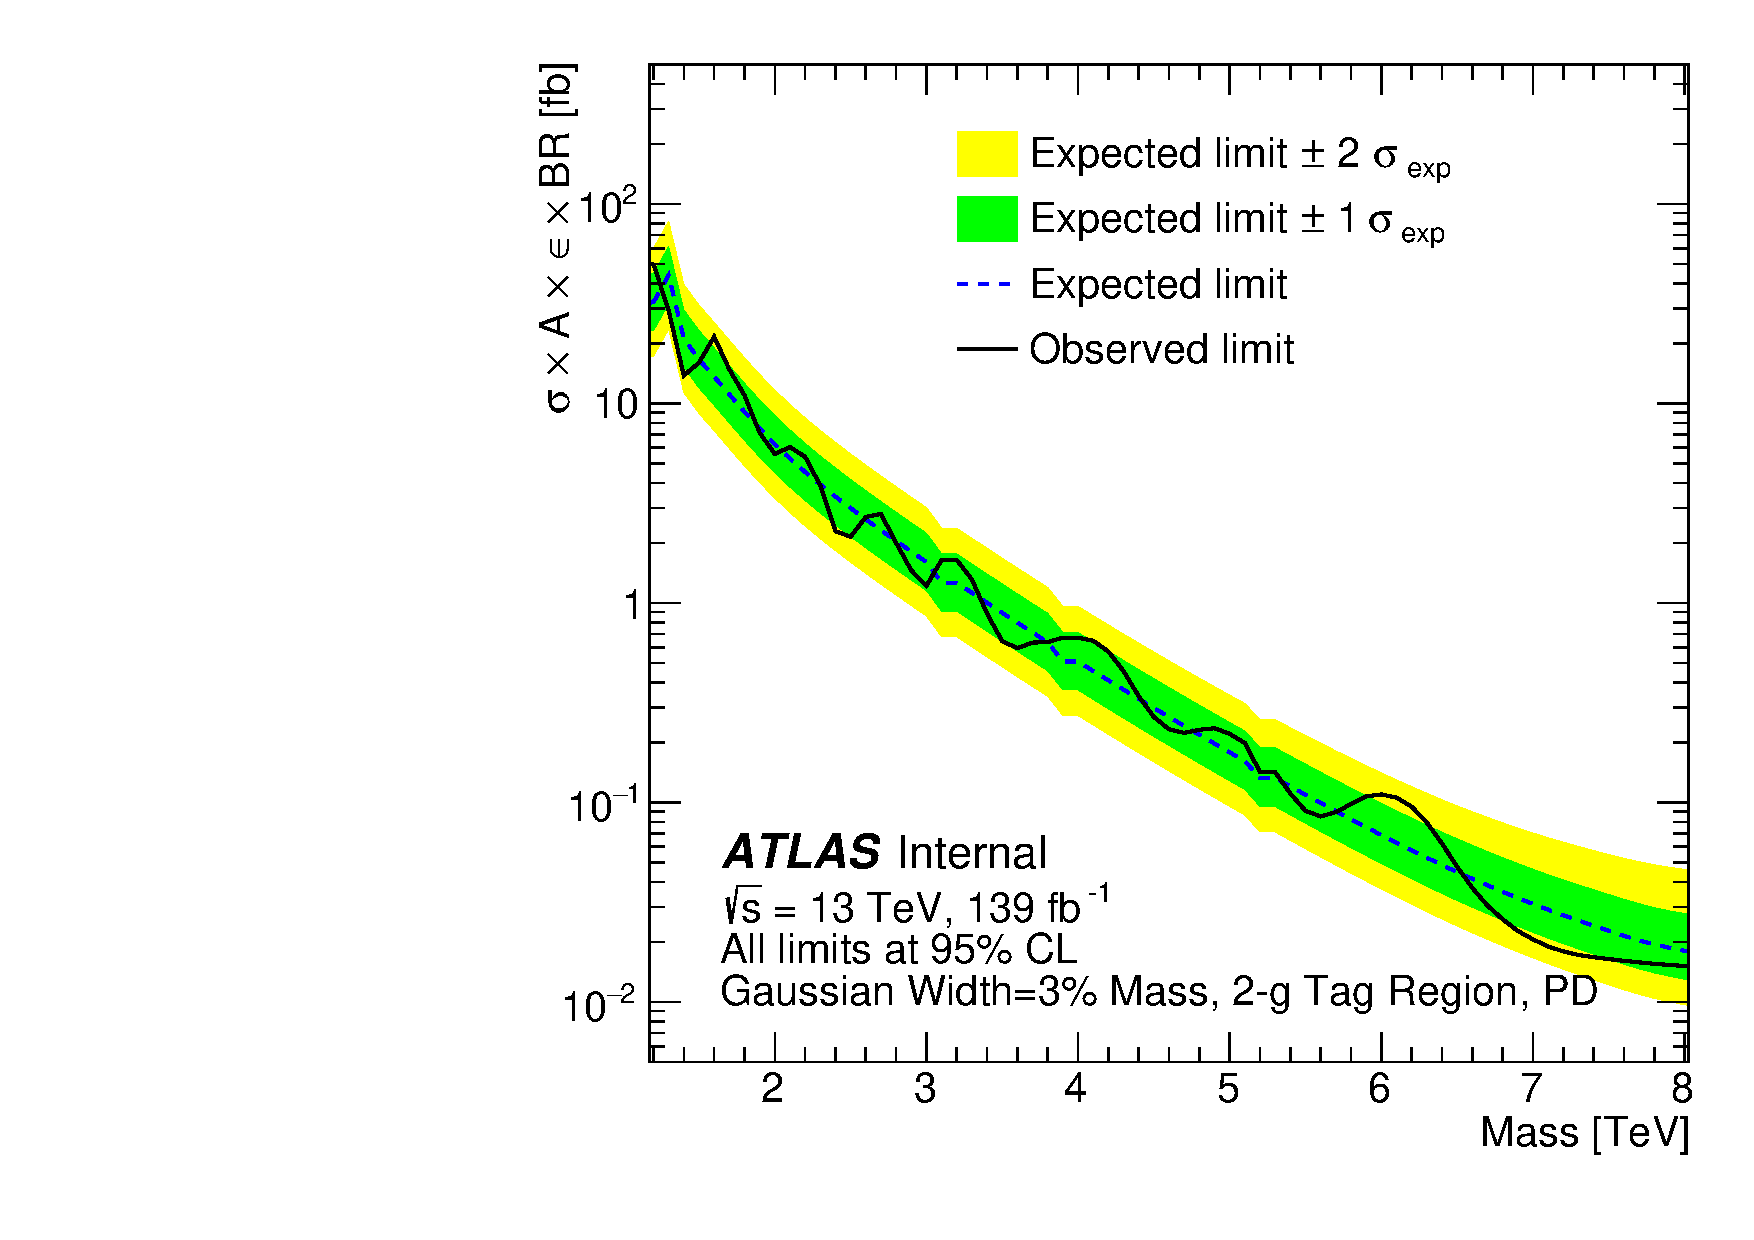
\includegraphics[width=0.4\textwidth]{fig/app-SignalIndependentLimits/Gauss_Limits_yStar0p8_Tag2_WidthPercent3_1200to8000_sigma.pdf}
%            }\\
%            \subfloat[5\% Width Gaussian Limits]{ 
%%                \label{fig:SignalIndependentGaussianLimits_SubWidth5} % uncomment if label used. 
%                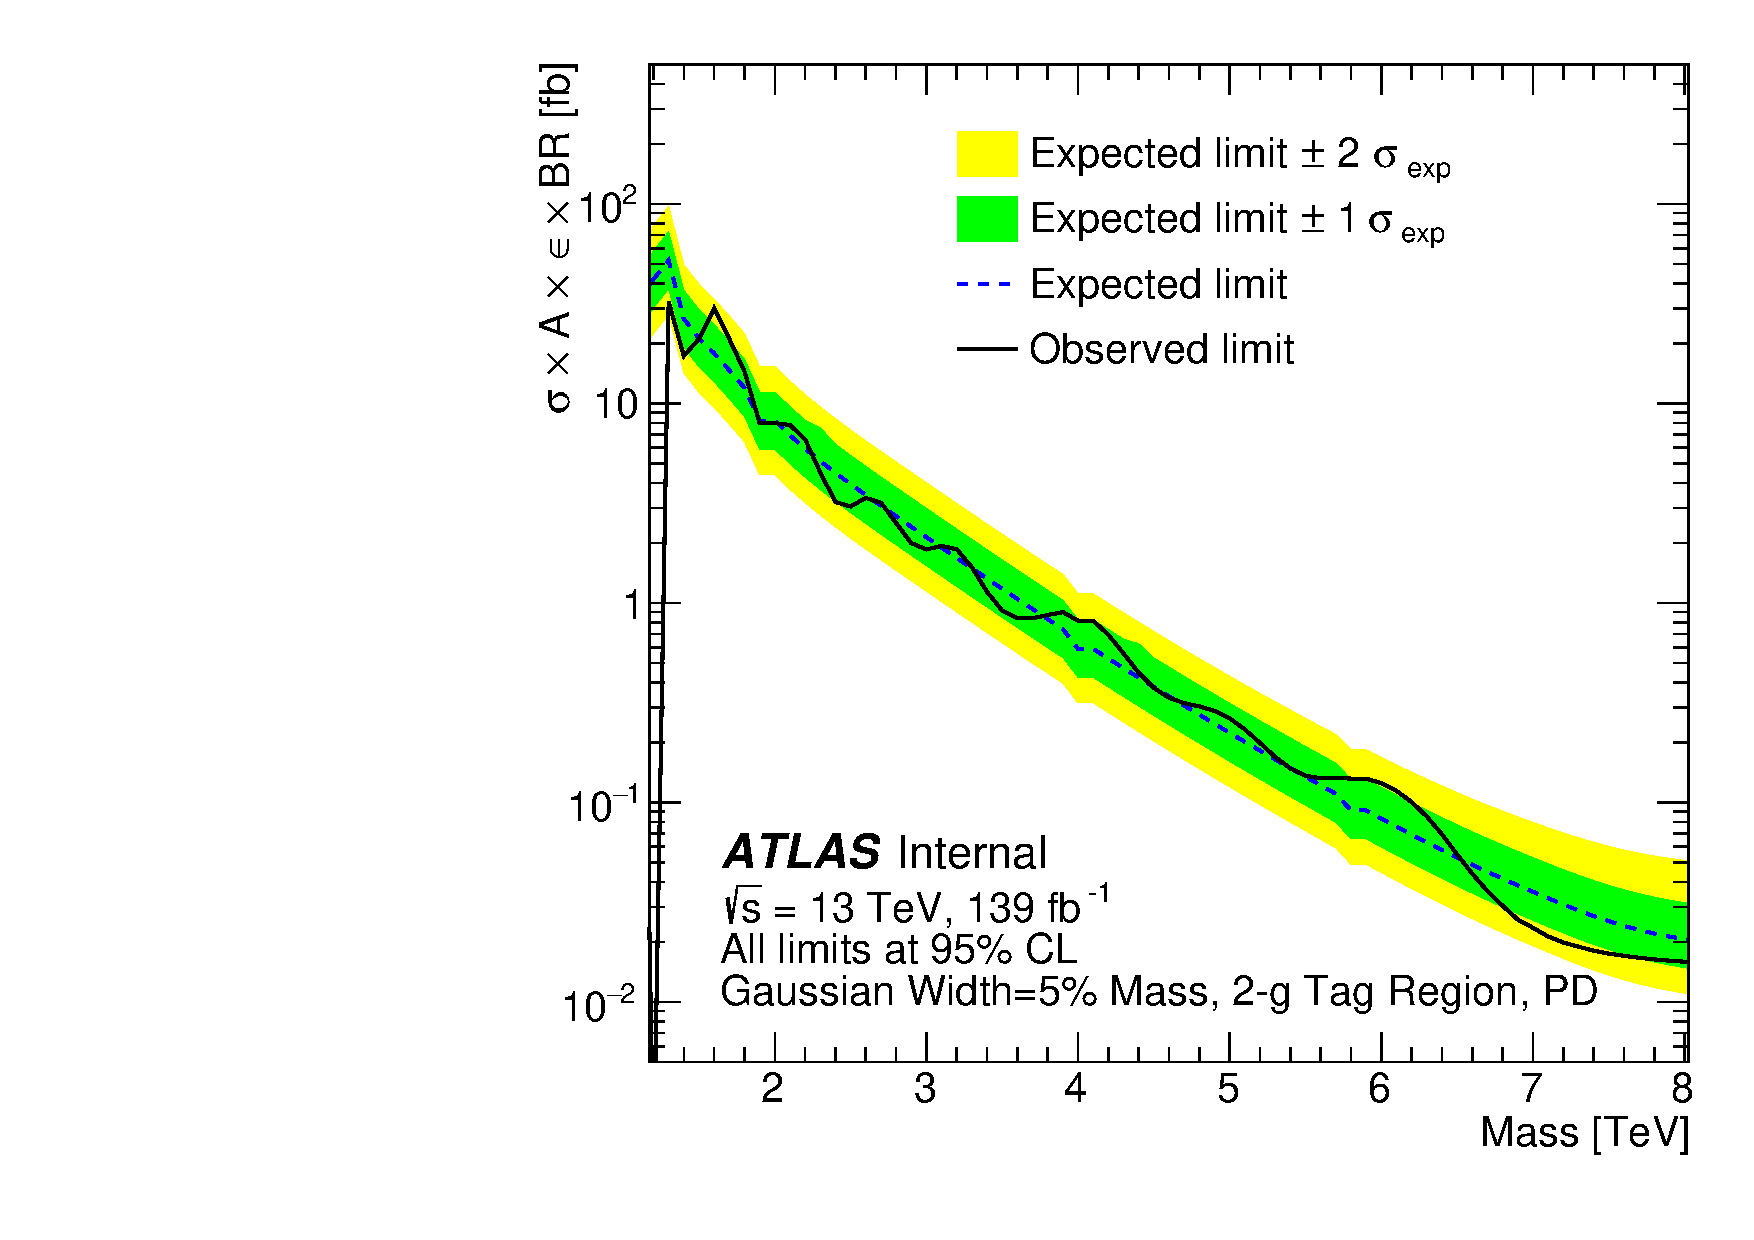
\includegraphics[width=0.4\textwidth]{fig/app-SignalIndependentLimits/Gauss_Limits_yStar0p8_Tag2_WidthPercent5_1200to8000_sigma.pdf}
%            }
%            \subfloat[7\% Width Gaussian Limits]{ 
%%                \label{fig:SignalIndependentGaussianLimits_SubWidth7} % uncomment if label used. 
%                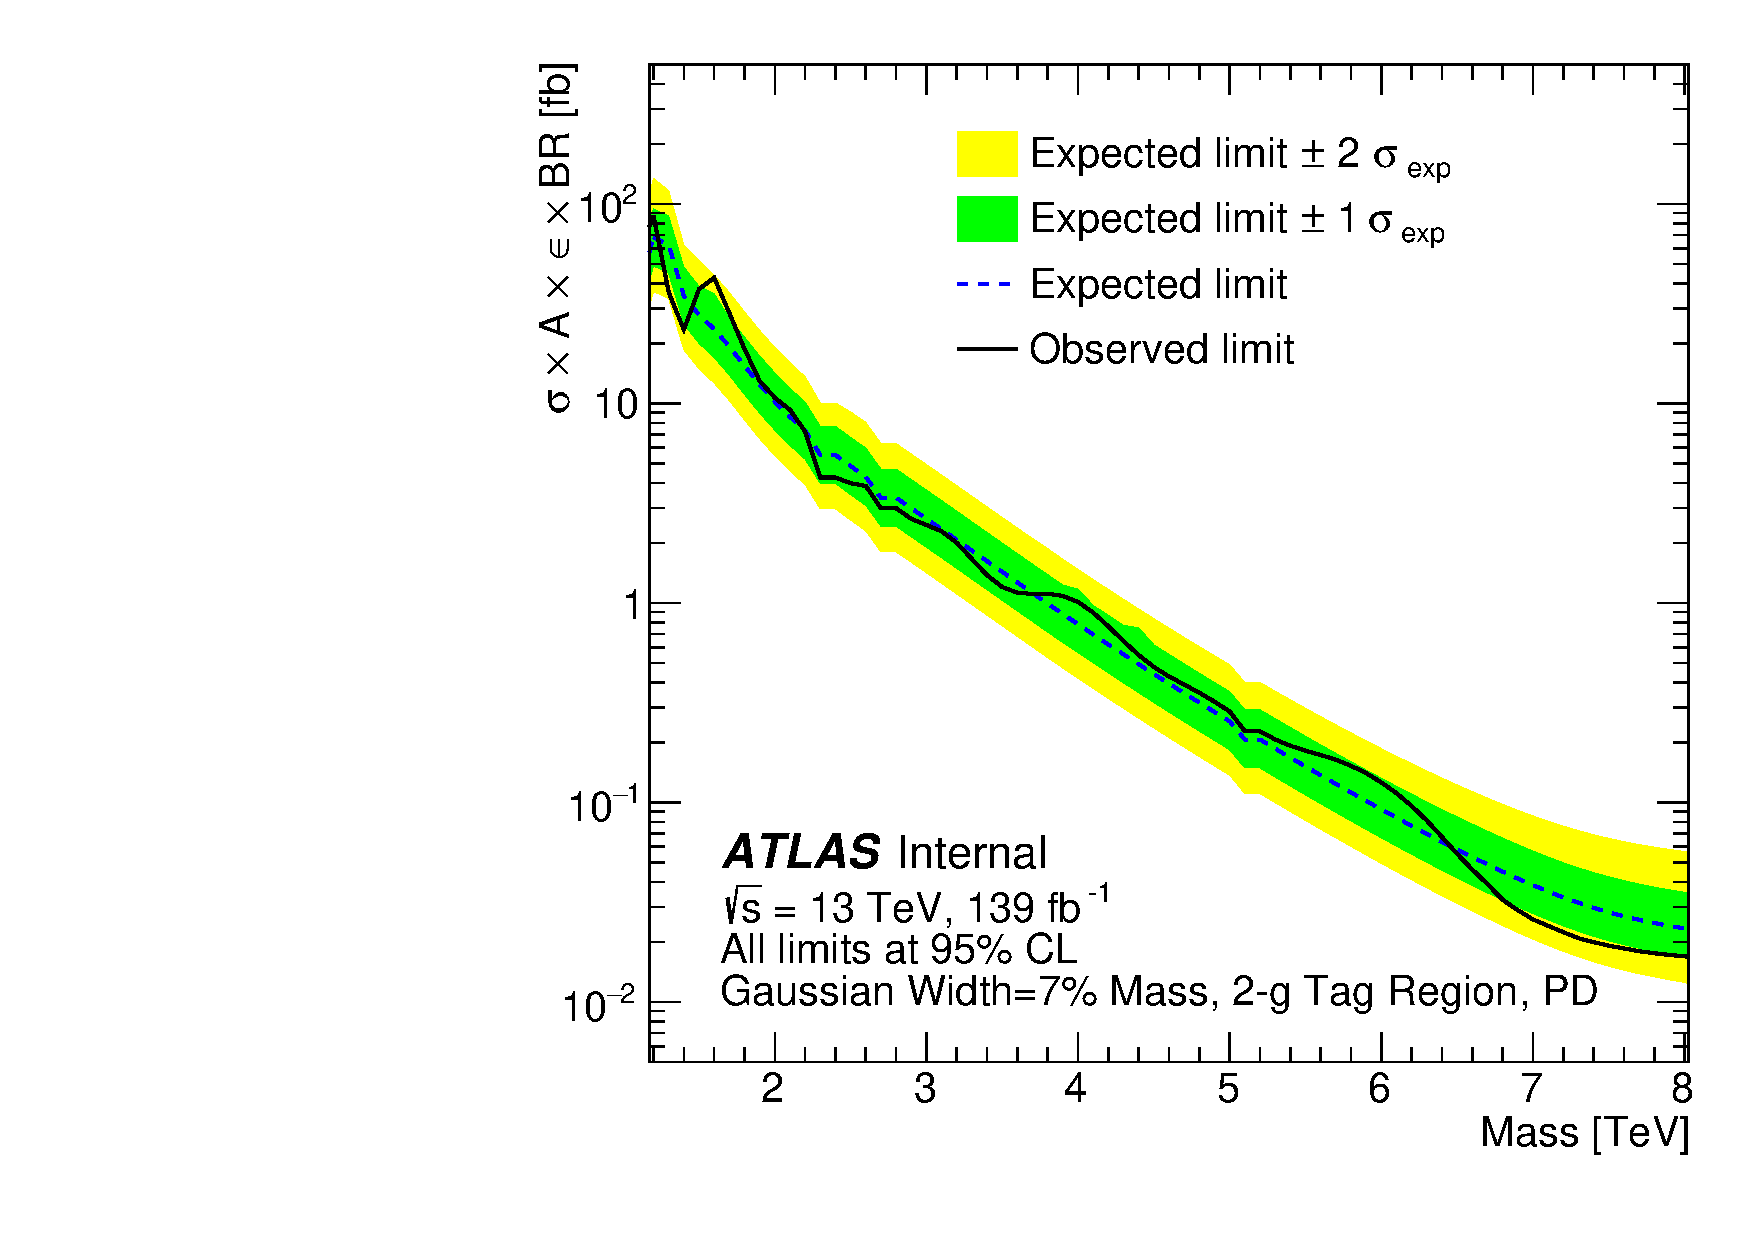
\includegraphics[width=0.4\textwidth]{fig/app-SignalIndependentLimits/Gauss_Limits_yStar0p8_Tag2_WidthPercent7_1200to8000_sigma.pdf}
%            }\\
%            \subfloat[10\% Width Gaussian Limits]{ 
%%                \label{fig:SignalIndependentGaussianLimits_SubWidth10} % uncomment if label used. 
%                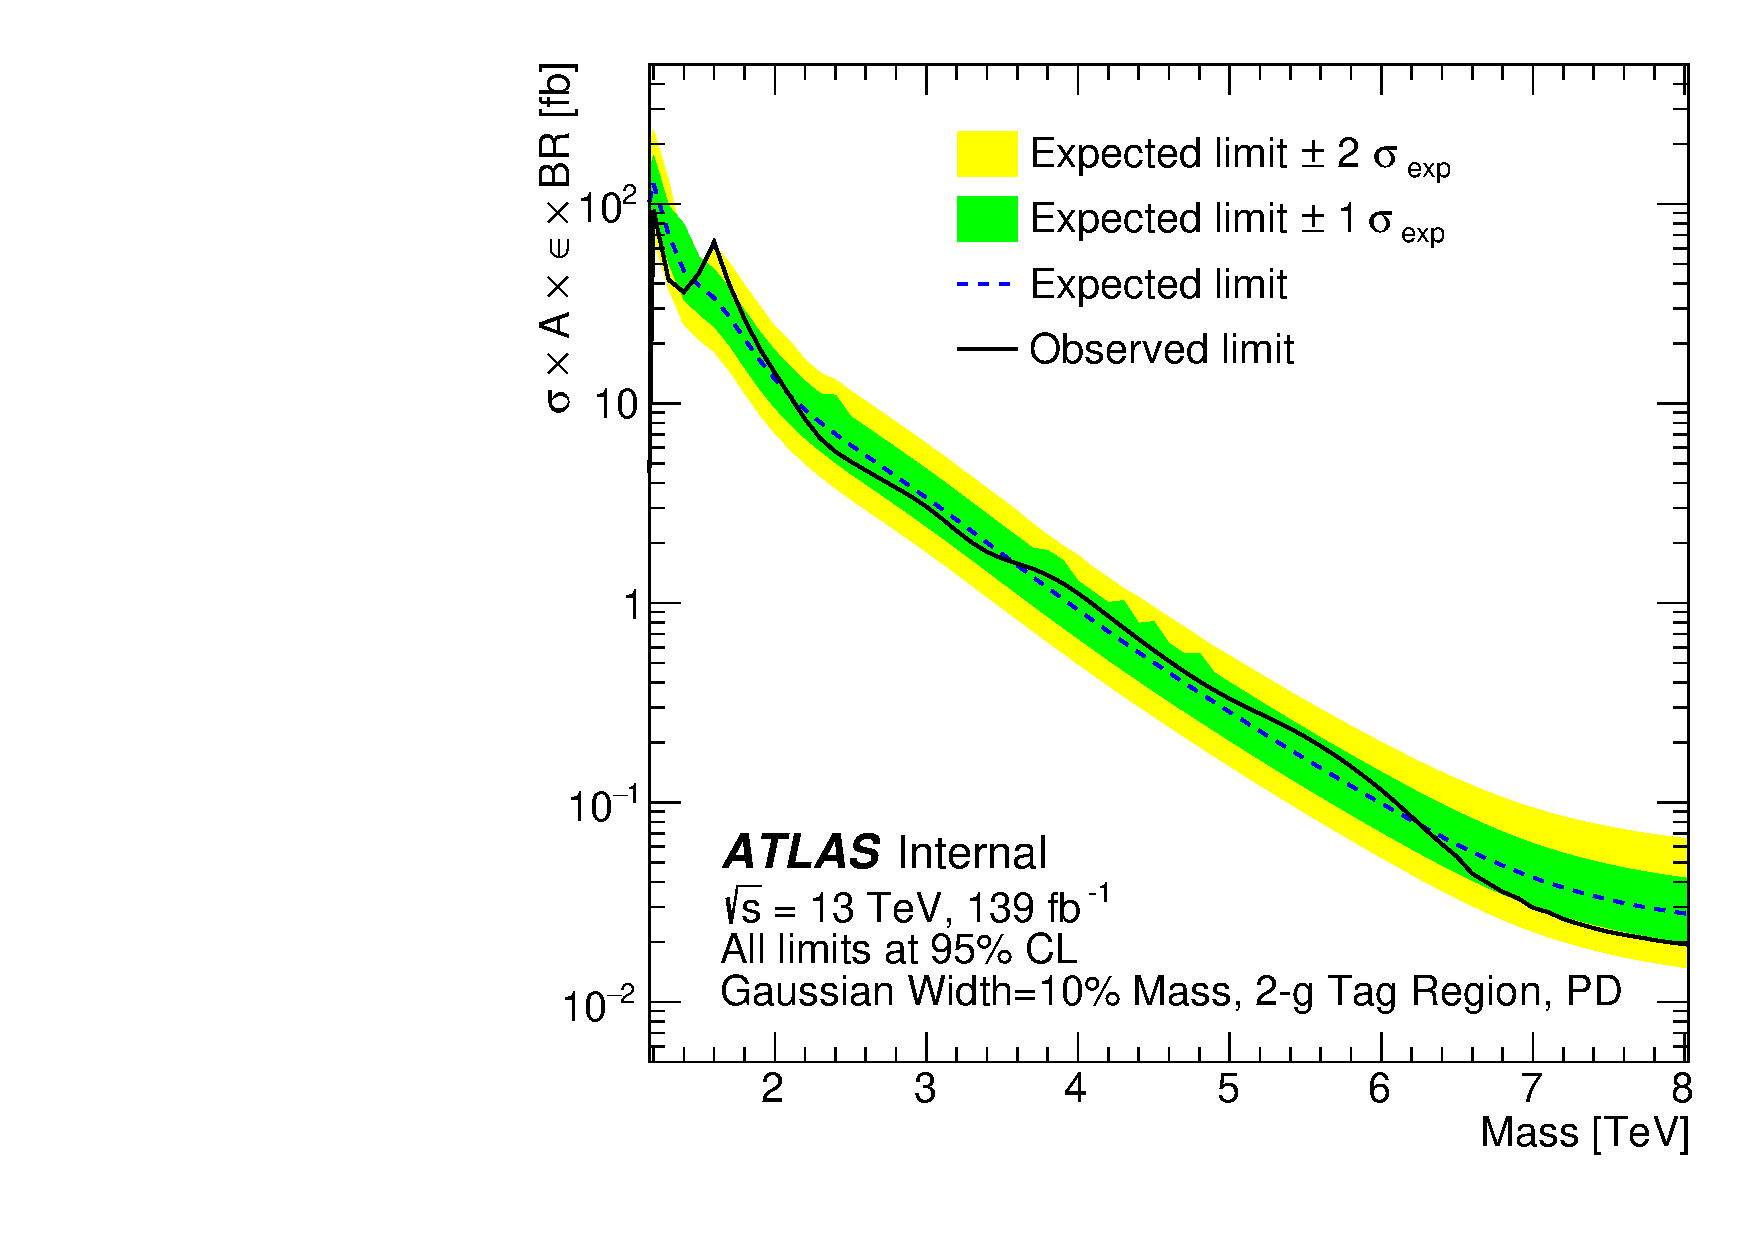
\includegraphics[width=0.4\textwidth]{fig/app-SignalIndependentLimits/Gauss_Limits_yStar0p8_Tag2_WidthPercent10_1200to8000_sigma.pdf}
%            }
%            \subfloat[15\% Width Gaussian Limits]{ 
%%                \label{fig:SignalIndependentGaussianLimits_SubWidth15} % uncomment if label used. 
%                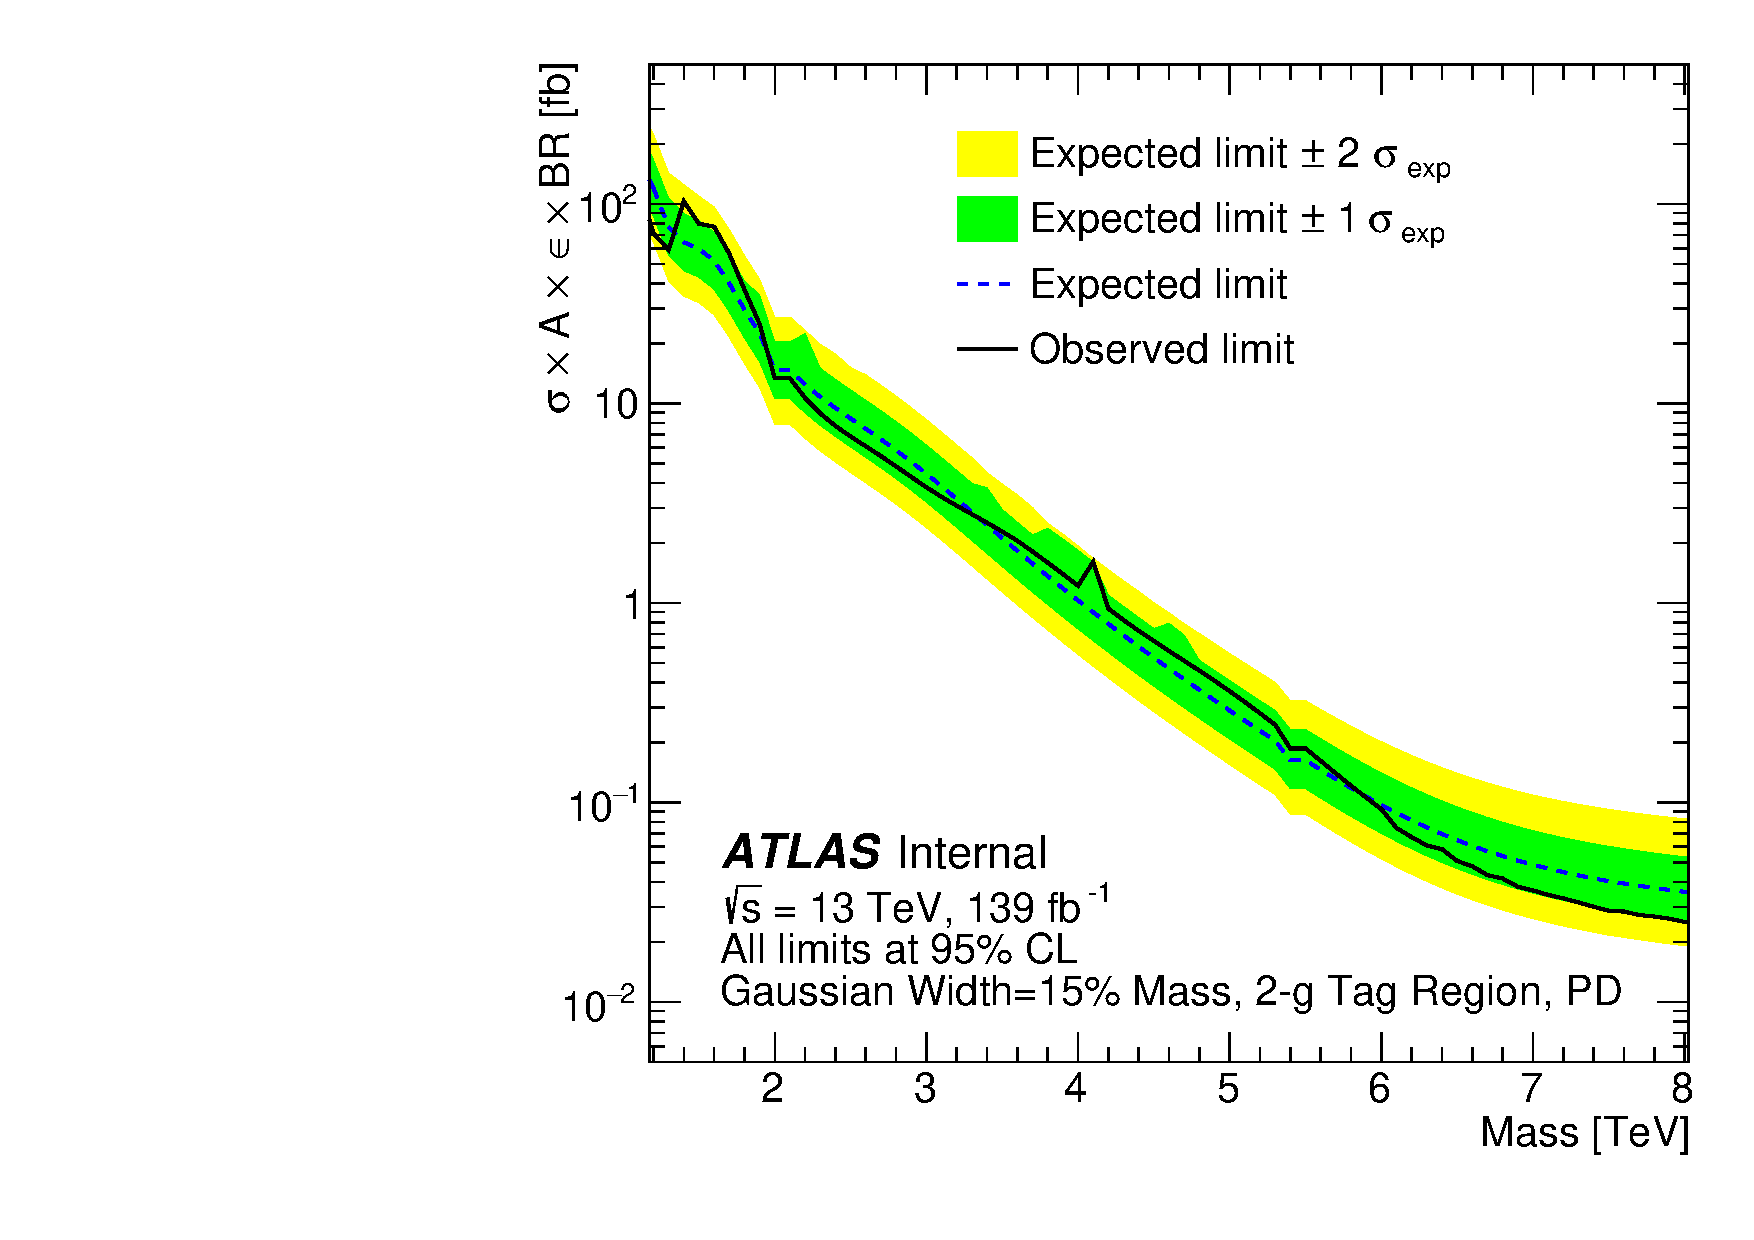
\includegraphics[width=0.4\textwidth]{fig/app-SignalIndependentLimits/Gauss_Limits_yStar0p8_Tag2_WidthPercent15_1200to8000_sigma.pdf}
%            }
%            \caption{Model-independent limits set in the 2-$g$ tagged $y^{*} < 0.8$ Signal Region using Gaussian resonances of varying widths from 0\% to 15\% of their peak position without systematics included using the full 139fb$^{-1}$ Run-2 dataset.}
%            \label{fig:SignalIndependentGaussianLimits_2gYStar0p8}
%        \end{figure}


